\documentclass[a4paper,12pt]{article}

\usepackage{titlesec}
\usepackage{hyperref}
\usepackage{amsmath}
\usepackage{amssymb}
\usepackage{braket}
\usepackage[utf8]{inputenc}
\usepackage{tikz}
\usepackage{cancel}
\usepackage[top=3cm, bottom=3cm, left=2cm, right=2cm]{geometry}
\usepackage{graphicx}
\usepackage{subcaption}
\usepackage{float}
\usetikzlibrary{arrows.meta, angles, quotes}

\allowdisplaybreaks

\titleformat{\section}
{\normalfont\normalsize\bfseries}
{\thesection}{1em}{}
\titleformat{\subsection}
{\normalfont\small\bfseries}
{\thesubsection}{1em}{}
\titleformat{\subsubsection}
{\normalfont\small\bfseries}
{\thesubsubsection}{1em}{}

\title{
	\vspace{2cm}
	\Huge \textbf{Collisional Methods by Francesco} \\[0.5cm]
	\large Collection of notes, formulas and demonstrations in the field of dynamics of open quantum systems and Collisional Methods
	\vspace{5cm}
}

\author{\Large Francesco Ciavarella - University of Padua \\[10pt] \href{mailto:francesco.ciavarella@studenti.unipd.it}{francesco.ciavarella@studenti.unipd.it}}

\begin{document}
	
	\maketitle
	\thispagestyle{empty} 
	\newpage
	
	\tableofcontents
	\newpage
	
	\section{Introduction}
	\label{sec:intro}
	
	\subsection{Open Quantum System an Quantum Master Equation}
	\label{sub:open_quantum_sys_QME}
	First, it is essential to frame the scope of this project within the field of \textit{Environment-Assisted Quantum Transport (ENAQT)}. This framework focuses on evaluating the effects of the surrounding environment on open quantum systems. The latter are usually constituted of a set of qubits representing different chromophores' energy states.
	Such systems are typically described using the \textit{density matrix} formalism, where we define $ \rho_S = \sum_{k}^{N}{\ket{\Psi_{k}^{S}}\bra{\Psi_{k}^{S}}} $.\\
	This approach is fundamental as it allows for the treatment of quantum systems subject to classical statistical uncertainty (i.e. mixed states), combining quantum coherent superposition with classical probabilities.
	
	Specifically, ENAQT explores how environment-induced phenomena can enhance the efficiency of excitonic transport across different sites (i.e., the transfer of excitation). In this context, one of the simplest environmental effects is the induction of \textit{Decoherence}: a mechanism that facilitates the transfer of excitation toward the final target site by destroying the coherence between different sites and localizing the excitation in a single one.
	
	In the study of open quantum systems, various equations can describe the dynamics of these sites, defined as the evolution of the system's density matrix over time.	
	
	To account for environmental effects, it would formally be necessary to study the evolution of the \textit{total system}, i.e. comprising both the sites and the environment's degrees of freedom, and subsequently perform a \textit{partial trace} over the latter. However, since the dimensionality of this total Hilbert space is often computationally unmanageable, the standard approach involves the use of \textit{Dynamical Maps}. These maps allow us to obtain the evolution of the system alone while still accounting for the effect of the external environment, such as \textit{Dephasing} or \textit{Relaxation}.
	
	Among the most well-known \textit{Dynamical Maps} there are the \textit{Redfield equation}, which is microscopically derived, and the \textit{Lindblad equation}. The latter is based on the theory of quantum semigroups and is derived with a more mathematical approach to ensure the evolution remains \textit{Completely Positive and Trace Preserving} (CPTP) at all times. In this work, we will specifically focus on the Lindblad master equation, which reads : 
	
	\begin{equation}
		\dot{\rho_{S}} = -i [\hat{H}, \rho_{S}] + \sum_j \gamma_j \left( \hat{L}_j \rho_{S} {\hat{L}_j}^\dagger - \frac{1}{2} \left[ \hat{L}_j^\dagger \hat{L}_j, \rho_{S} \right]_{+} \right) = \hat{\mathcal{L}} \rho_{S}
		\label{eq:lindblad}
	\end{equation}
	
	where $ \gamma_j $ are the \textit{Lindblad rates}, that may be different for every sites; while $ \hat{L}_j $ are the \textit{Jump operator}, which describe the environment effect on the system; eventually $ \hat{\mathcal{L}} $ represents the \textit{Liouvillian Super Operator}.
	
	In this specific study, we will focus exclusively on the phenomenon of \textit{pure Dephasing}. This process is responsible for the suppression of quantum coherences between different sites, favoring excitonic transport. 
	For our model, this mechanism is described by the jump operators 
	\begin{equation}
		\hat{L}_j = \sigma_z^{(k)}
		\label{eq:jump_operator_z}
	\end{equation}
	where $\sigma_z$ is the Pauli matrices acting on the $k$-th site (represented by a qubit). This choice of operator ensures that while the off-diagonal elements of the density matrix (the coherences) decay over time, the diagonal elements (the populations) remain unaffected.
	
	\subsection{Lindblad Evolution}
	\label{sub:lindblad_evo}
	We will study the dynamic represented with a Lindblad equation of the density matrix of an excitonic dimer.We'll use an initial Density Matrix which only has population in the first site: 
	\begin{equation}
		\rho (0)  = \begin{bmatrix}1 & 0 \\ 0 & 0 \\\end{bmatrix}
	\end{equation}
	The Lindblad equation reads:
	\begin{equation}
		\frac{d}{dt} \rho (t) = 	-\frac{i}{\hbar} \left[ \hat{H}, \rho (t) \right] + \sum_{j}{\gamma_j \left( \mathcal{L}_j \rho (t) \mathcal{L}_j^\dagger - \frac{1}{2} \left[ \mathcal{L}_j^\dagger \mathcal{L}_j, \rho (t) \right]_+ \right) }
	\end{equation}
	
	At first we'll study the \textit{Pure Dephasing} effect, obtained with $ \mathcal{L}_{k} = \sigma_{z} $
	
	complete ...
	
	\newpage
	
	\subsection{Stochastic Unraveling of Quantum Master Equation}
	\label{sub:unraveling}
	
	The concept of \textit{unraveling} refers to the decomposition of the deterministic Master Equation into a statistical ensemble of single stochastic trajectories. Instead of directly evolving the density matrix $ \rho_{S} $, which describes the average state of the ensemble, one evolves a single wave function $ \ket{\psi(t)} $ subject to random events, which represents the direct effect of the environment on the quantum state. The full dynamics of the density matrix is then reconstructed by averaging over a large number of these realizations:
	\begin{equation}
		\rho_{S}(t) \approx \frac{1}{M} \sum_{j=1}^M \ket{\psi_{j}^{S}(t)}\bra{\psi_{j}^{S}(t)}
		\label{eq:mean_over_traj}
	\end{equation}
	where $M$ is the number of simulated trajectories.
	
	This approach offers different advantages such as the reduction of the computational cost, since with if $N$ is the dimension of the Hilbert space, the density matrix $\rho$ involves $N^2$ elements and it's evolution scales as $O(N^2)$, instead of the wave function, that contains only $N$ components and scales as $O(N)$. \\
	Another advantage is that the Master Equation describes only the average effect of the environment on the System Density Matrix, while in the stochastic unraveling, analyzing a single realization, it's possible to understand how effectively the environment affects the system, distinguishing between the fundamental quantum uncertainty and the statistical mixture resulting from decoherence.
	
	In this sense it's possible to define two opposite limits, describing the  environment effect on the system, which are the so called :
	
	\begin{itemize}
		\item \textbf{Diffusive Limit:} The environment induces small changes in the system's state but acts continuously in time, behaving as a source of random noise. This regime is physically associated with a \textit{weak measurement} performed on the system.
		
		\item \textbf{Quantum Jump Limit:} The environment induces a strong, discontinuous modification of the system's wave function, but the probability of this event occurring is very low in a single time step. In contrast to the diffusive case, this limit corresponds to a \textit{strong measurement} performed on the system.
	\end{itemize}
	
	\subsection{Collisional Method}
	\label{sub:CM}
	While there are several established algorithms for unraveling the Quantum Master Equation—such as the \textit{Stochastic Schr\"odinger Equation} (SSE) or the \textit{Monte Carlo Wave Function} (MCWF) method, this work focuses on the \textit{Collisional Model} framework.
	
	The primary objective is to implement and explore this approach, which reconstructs the continuous dynamics through a sequence of discrete interactions, called \textit{Collisions}, occurring over a finite time step $\Delta t$.
	In this model, the environment is not treated as a continuum but is represented by a set of auxiliary units called \textit{Ancillas}, typically modeled as qubits (two-level systems).
	
	The dynamics proceeds as follows:
	\begin{enumerate}
		\item \textbf{Initialization:} At the beginning of each step, the System and the current Ancilla are in a \textit{product state}, $\rho_{tot} = \rho_S \otimes \rho_A$.
		\item \textbf{Collision:} They undergo a joint unitary evolution governed by a specific \textit{Collisional Hamiltonian}, which generally creates entanglement between the System and the Ancilla.
		\item \textbf{Measurement:} A measurement is performed on the Ancilla. Due to the quantum correlations established during the collision, the outcome of this measurement induces a conditional change on the System's state.
		\item \textbf{Reset:} After the measurement, the current ancilla is discarded. For the next time step, the system interacts with a new, identical ancilla initialized in the same initial state, and the cycle repeats. This ensures the Markovian nature of the dynamics. 
	\end{enumerate}
	
	Since the probability of measuring one of the two Ancilla's states is finite, it is possible to implement a \textit{Stochastic Algorithm} which randomly chooses the change to apply to the System, according to the Ancilla's measurement outcome. In this way, it is possible to obtain a single \textit{Random Trajectory}.
	
	But first of all, focus on the Collisional Methods Hamiltonian form, which in general is divided in two term :
	\begin{equation}
		\mathcal{H}_{CM} = \mathcal{H}_{Exc} + \mathcal{H}_{Collision}
		\label{eq:CM_hamiltonian}
	\end{equation}
	where 
	\begin{equation}
		\mathcal{H}_{Exc} = \mathcal{H}_{Site} + V_{Hopping} = \sum_{j=1}^{N} {\frac{\varepsilon_j}{2} \sigma_{z}^{j} \otimes \mathbb{I}^{\otimes N} } + \sum_{\langle j,j' \rangle} {\frac{V_{j,j'}}{2} \left( \sigma_{x}^{j}\sigma_{x}^{j'} \otimes \mathbb{I}^{\otimes N} + \sigma_{y}^{j}\sigma_{y}^{j'} \otimes \mathbb{I}^{\otimes N} \right)}
		\label{eq:Exc_Hamiltonian} 
	\end{equation}  represents the \textit{Isolated System Hamiltonian},representing the internal dynamics of the $N$ sites.The Hopping term specifically is what allows the effective Exciton transfer, since the Collisonal term just facilitates the transport by canceling the coherence created. The summation on \textit{j} runs over the different System's sites and the  $ \sigma_{\alpha}^j $ term are defined as :
	\begin{equation}
		\sigma_{\alpha}^j  = \mathbb{I}^{\otimes j-1} \otimes \sigma_{\alpha} \otimes \mathbb{I}^{\otimes N-j}
		\label{eq:sigma_op_definition}
	\end{equation}
	
	The form of $ \mathcal{H}_{Collision} $ specifically defines the unraveling regime. In order to recover the correct QME form, it's fundamental to correctly initialize the Ancilla's state, which is deeply related to the specific form of \textit{Interaction Hamiltonian}, $ \mathcal{H}_{Collision} $. \\	
	In this context it's possible to associate the two opposite regime, seen before, with two different configurations of the Collisional Method ( i.e. form of the Collisional Hamiltonian and Ancilla's state initialization ): 
	
	\begin{description}
		\item[Diffusive Limit]
		\begin{equation}
			\mathcal{H}_{Coll} = \sum_{j=1}^{N}{c_j \sigma_{z}^{j} \otimes \sigma_{z}^{a_j}} \text{\quad and \quad} \rho_{A} = \frac{1}{2} \begin{pmatrix} 1 & 0 \\ 0 & 1 \end{pmatrix}
			\label{eq:diff_initialization}
		\end{equation}
		The Ancilla is in the complete mixed state, i.e. given a reservoir of Ancillas, there's the 0.5 probability of finding it in the $ \ket{0_a} $ state and so the same for $ \ket{1_a} $ state; in this case  the $ \mathcal{H}_{Coll} $ acts on the Ancilla as a $ \sigma_{z}^{a_j} $, introducing a phase shift on the sate.
		\item[Quantum Jump Limit] 
		\begin{equation}
			\mathcal{H}_{Coll} = \sum_{j=1}^{N}{c_j \sigma_{z}^{j} \otimes \sigma_{x}^{a_j}} \text{\quad and \quad} \rho_{A} = \begin{pmatrix} 1 & 0 \\ 0 & 0 \end{pmatrix}
			\label{eq:QJ_initialization}
		\end{equation}
		The Ancilla is always initialized in the $ \ket{0_a} $ state and the $ \mathcal{H}_{Coll} $ acts on it as a $ \sigma_{x}^{a_j} $ flipping its state.
	\end{description}
	In both cases $ c_j $ represents the \textit{Collision Intensity} for every \textit{j-th} site, a constant related to the \textit{Lindblad Rates} $ \gamma_j $ by the equation:
	\begin{equation}
		c_j = \sqrt{\gamma_j / 4\Delta t}
		\label{eq:c_j_definition} 
	\end{equation}
	
	
	Once we've defined the $ \mathcal{H}_{Collision} $, it's important to see how it affect the System's evolution. In general the wave function at a time step $ t + \Delta t $ is given by the resolution of the Schr\"odinger Equation, which is :
	\begin{equation}
		\ket{\Psi_S (t + \Delta t)} = \mathcal{U} \ket{\Psi_S (t)} = e^{\left(-i \, \mathcal{H}_{CM} \Delta t\right)}\ket{\Psi_S (t)} = e^{\left(-i \, \mathcal{H}_{Exc} \Delta t\right)} e^{\left(-i \, \mathcal{H}_{Coll} \Delta t\right)}\ket{\Psi_S (t)} 
		\label{eq:wf_evolution}
	\end{equation}
	where the last equivalence is valid thanks to a \textit{Trotter-Suzuki} decomposition and allows to separate the evolution in two step:
	\begin{enumerate}
		\item Isolated evolution via $ \mathcal{H}_{Exc} $
		\item Collisional evolution via $ \mathcal{H}_{Coll} $
	\end{enumerate}
	Focusing on the collisional evolution we can analytically define the Evolution Operator \textit{U} form and how it modifies the System \textit{wf}, in the two different limits. Note that in this derivation we will refer to only one site of the System's Hilbert space:
	
	\begin{description}
		\item[Diffusive Limit] 
		\begin{equation}
			U_{collsion} = \exp \left(-i c_j \sigma_{z}^{j} \otimes \sigma_{z}^{a_j} \Delta t\right) = \cos \left(c_j \Delta t \right) \mathbb{I}^j \otimes \mathbb{I}^a - i \sin \left(c_j \Delta t \right) \sigma_{z}^{j} \otimes \sigma_{z}^{a_j}
			\label{eq:U_coll_Diff}
		\end{equation}
		In this case, since we have to deal with a completely mixed Ancilla's Density Matrix we divide the evolution in two different results based on the Ancilla's state, including in this sense the Classical uncertainty, which is $0.5$ for both the states:
		\begin{align}
			\ket{\Psi_0 (t + \Delta t) } = \Big[ \cos \left(c_j \Delta t \right) - i \sin \left(c_j \Delta t \right) \sigma_{z}^{j} \Big] \ket{\Psi_S(t)} \otimes \ket{0_a}
			\label{eq:psi_evol_Diff0} \\
			\ket{\Psi_1 (t + \Delta t) } = \Big[ \cos \left(c_j \Delta t \right) + i \sin \left(c_j \Delta t \right) \sigma_{z}^{j} \Big] \ket{\Psi_S(t)} \otimes \ket{1_a} 
			\label{eq:psi_evol_Diff1}
		\end{align}
		Depending on the ancilla's state, the system undergoes a rotation in the opposite direction in the Hilbert space; specifically, if the ancilla is in $ \ket{0_a} $ the phase shift is $ + c_j \Delta t \sigma_{z}^{j} $, whereas with $ \ket{1_a} $ the phase shift is $ - c_j \Delta t \sigma_{z}^{j} $. This stochastic alternation between opposite phase shifts results in a quantum random walk of the system's phase. In the limit $ \Delta t \rightarrow 0 $, this discrete process converges to a continuous Brownian motion (Wiener process). Since $ \Delta t \rightarrow 0 $ the effect on the system will be very small.
		\item[Quantum Jump Limit] 
		\begin{equation}
			U_{collsion} = \exp \left(-i c_j \sigma_{z}^{j} \otimes \sigma_{x}^{a_j} \Delta t\right) = \cos \left(c_j \Delta t \right) \mathbb{I}^j \otimes \mathbb{I}^a - i \sin \left(c_j \Delta t \right) \sigma_{z}^{j} \otimes \sigma_{x}^{a_j}
			\label{eq:U_coll_QJ}
		\end{equation}
		\begin{equation}
			\ket{\Psi (t + \Delta t) } = \cos \left(c_j \Delta t \right) \ket{\Psi_S (t)} \otimes \ket{0_a} - i \sin \left(c_j \Delta t \right) \sigma_{z}^{j} \ket{\Psi_S(t)} \otimes \ket{1_a}
			\label{eq:psi_evol_QJ}
		\end{equation}
		In this case we have a modification on the System \textit{wf} only when we measure $ \ket{1_a} $, but the variation isn't premultiplied by a small factor so the change will be significant. On the other hand the probability of measuring $ \ket{1_a} $ is given by
		\begin{equation}
			P_{1_a} = Tr_S \Big[\braket{1_a | \Psi(t + \Delta t)}\braket{\Psi(t + \Delta t) | 1_a}\Big] = \sin^{2}{\left(c_j \Delta t\right)}
			\label{eq:ancilla_probability}
		\end{equation} 
		So in this case we have a significant variation but that happens very rarely.
	\end{description}  
	For more information about the equation derivation please see the \href{run:./Demonstration.pdf}{Demonstration file}, in particular section 1.1 and 2.1. Moreover all the form of $ \ket{\Psi (t + \Delta t) } $ can be lead back to a Lindblad evolution, as specified in section 1.3 and 2.3
	
	\subsection{Theoretical Algorithm}
	\label{sub:theoretical_algorithm}
	Concatenating the evolution given by Eq.\eqref{eq:psi_evol_Diff0} and Eq.\eqref{eq:psi_evol_Diff1} or Eq.\eqref{eq:psi_evol_QJ}, it's possible to create a Stochastic Algorithm that creates a Trajectory in the two limits; averaging then different trajectories realizations it's possible to recover the Lindblad evolution.
	
	\begin{description}
		\item[Quantum Jump Algorithm] \leavevmode
		\begin{enumerate} 
			\item Isolated System's evolution with $ \mathcal{U}_{Exc} = \exp{\left( -i \, \mathcal{H}_{Exc} \Delta t \right) }$
			\item Extraction for every different site of a Random Number $\alpha$ in $[0,1]$
			\item If $ \alpha < \sin^{2}{\left(c_j \Delta t\right)} $ it means that there's been an effective collision that has flipped the initial Ancilla's state $ \ket{0_a} $ to $ \ket{1_a} $ and so the System's \textit{wf} gets modified by $ \sigma_{z}^{j} $ on every \textit{j-th} site; \\
			if $ \alpha > \sin^{2}{\left(c_j \Delta t\right)} $ the system remain unchanged (i.e. application of $ \mathbb{I}^j $ )
			\item Once all the sites have been processed , measure and store System's Observables at that time step (like population)
			\item Repeat the algorithm for the next time step
		\end{enumerate}
		\item[Diffusive Algorithm] \leavevmode
		\begin{enumerate} 
			\item Isolated System's evolution with $ \mathcal{U}_{Exc} = \exp{\left( -i \, \mathcal{H}_{Exc} \Delta t \right) }$
			\item Extraction for every different site of a Random Number 	$\alpha$ in $[0,1]$
			\item If $ \alpha < 0.5 $ it means that state $ \ket{0_a} $ has been measured and so the System's \textit{wf} gets modified via EQ.\eqref{eq:psi_evol_Diff0} for every \textit{j-th} site;
			otherwise state $ \ket{1_a} $ has been measured and the System's \textit{wf} gets modified via EQ.\eqref{eq:psi_evol_Diff1}.
			\item Once all the sites have been processed , measure and store System's Observables at that time step (like population)
			\item Repeat the algorithm for the next time step
		\end{enumerate}
	\end{description}
	
	Since the update operators in both limits are unitary, the wave function norm is theoretically preserved at each step. However, to prevent numerical errors from accumulating over long simulations, it is standard practice to enforce renormalization after every time step.
	
	\subsection{Complete Evolution and Ancilla Trace}
	\label{sub:complete_evolution}
	While the stochastic unraveling focuses on individual trajectories of the \textit{wf}, the \textit{Collisional Mode}l can also be formulated deterministically for the complete Density Matrix $ \rho_S \otimes \rho_A $. \\
	The evolution of the system's Density Matrix $\rho_S$ over a time step is obtained by evolving the total state and then performing a \textit{partial trace} over the Ancilla's degrees of freedom. This operation mathematically corresponds to averaging over all possible measurement outcomes of the ancilla. \\
	In this way we are creating a so called \textit{Dynamical Map} $ \Phi $, which reads:
	
	\begin{equation}
		\rho_S(t + \delta t) = \Phi[\rho_S(t)] = \text{Tr}_A \left[ \mathcal{U} \left( \rho_S(t) \otimes \rho_A \right) \mathcal{U} ^\dagger \right]
		\label{eq:dynamical_map}
	\end{equation}
	Since $\mathcal{U}$ is unitary, this map is guaranteed to be Completely Positive and Trace Preserving (CPTP).\\
	It can be shown that in the continuous limit, i.e $ \Delta t \rightarrow 0 $ the discrete map defined in Eq.\eqref{eq:dynamical_map} converges to the differential Lindblad Master Equation (see section 1.3 in \href{run:./Demonstration.pdf}{Demonstration file}). \\
	Thus, the Collisional Model serves as a rigorous microscopic derivation of the Lindblad dynamics.
	
	\section{Case Study : Exciton Dimer}
	\label{sec:exciton_dimer}
	Since this work is a preliminary study of \textit{Collisional Methods}, the system consider is one of the simplest relevant to quantum transport: the \textit{Exciton Dimer}. This system consists of two sites, where each site is modeled as a two-level system (qubit). The computational basis for the composite Hilbert space is given by: 
	\begin{equation}
		\left\{\ket{00}, \ket{01}, \ket{10}, \ket{11} \right\}
	\end{equation}
	where the notation $\ket{s_1 s_2}$ represents the tensor product $\ket{s}_1 \otimes \ket{s}_2$, with $0$ denoting the ground state and $1$ the excited state. \\
	Since the objective is to study the exciton transport between sites, the initial state is define as one site completely in excited state and the other in ground state. The interaction between the two sites is defined by the Hopping Potential \textit{v}, built to allow only exchange between the two excited states, conserving the total number of excitations. In this way
	the dynamics is restricted to the \textit{single-excitation manifold} and  allows us to effectively reduce the four-dimensional Hilbert space to a two-dimensional subspace, that can be represented by a single qubit built on the excited states $ \left\{ \ket{01}, \ket{10} \right\} $.
	As already said, the effect induced by the environment is just the \textit{Pure Dephasing}, which essentially destroys the coherence between the two states, facilitating the localization of the exciton.  
	
	The key observables analyzed during the time evolution are the Excited States Populations, representing the probability of finding the Excitation in site 1 or 2. Furthermore it's possible to reconstruct the the state vector in the \textit{Bloch Sphere}, which could help visualizing the evolution in time. 
	
	The results obtained with the \textit{Collisional Method}, both the Stochastic Trajectories and the Average Dynamics of the $ \rho_S $ (obtained tracing out the Ancilla), will be compared with the Lindblad Master Equation and the Isolated System Dynamics.
	
	\newpage
	
	\section{Quantum Jump limit in Collisional Methods}
	\label{sec:Quantum_Jump_limit_in_Collisional_Methods}
	\subsection{Evolution Operator and Ancilla Initialization}
	\label{sub:Evolution_Operator_and_Ancilla_Initialization_QJ}
	The goal is to reproduce the Lindbald dynamic using a Collsional Model, that gives us a trajectory of evolution of a single state of the density matrix $ \ket{\Psi_k} $ rappresentig a qubit. By repeting the dynamic several times it's possibile to recrate the Lindblad evolution of the density matrix.
	Different unravelling of the $ \rho (t) $ can be achieved by using different Collsional Hamiltonian. First we will reproduce the so called "Quantum Jump" or "Monte Carlo" limit, in which essentially the ancilla states stochastically jumps between the states $ \ket{0_a} $ and $ \ket{1_a} $ with a small probability to move to $ \ket{1} $ related to an effective collision, wich corresponds to an application of a $ \sigma_{z} $ to the system's state. \\
	The associated Hamiltonian acting on the System-Ancilla states is:
	\begin{gather}
		\mathcal{H}_{CM} = \mathcal{H}_{exc} + \mathcal{H}_{collision} \\
		= \sum_{j=1}^{N} {\frac{\varepsilon_j}{2} \sigma_{z}^{j} \otimes \mathbb{I}^{\otimes N} } + \sum_{\langle j,j' \rangle} {\frac{V_{j,j'}}{2} \left( \sigma_{x}^{j}\sigma_{x}^{j'} \otimes \mathbb{I}^{\otimes N} + \sigma_{y}^{j}\sigma_{y}^{j'} \otimes \mathbb{I}^{\otimes N} \right)} + \sum_{j=1}^{N}{c_j \sigma_{z}^{j} \otimes \sigma_{x}^{a_j}}
		\label{eq:CM_hamiltonian_QJ}
	\end{gather}
	where $ \sigma_{\alpha}^j = \mathbb{I}^{\otimes j-1} \otimes \sigma_{\alpha} \otimes \mathbb{I}^{\otimes N-j}  $ . \\
	The collision force $ c_j $ is related to the Lindblad phase shift constant by the equation $ c_j = \sqrt{\gamma_j / 4 \Delta t} $. 
	Let's focus on the Interaction Hamiltonian and how it acts on an already enatgled system-ancilla states $ \ket{\Psi} = \ket{\Psi_S} \otimes \ket{0_a} $ \\
	\\
	The evolution operator based on $ \mathcal{H}_{collsion} $ is :
	\begin{equation}
		U_{collsion} = \exp \left(-i c_j \sigma_{z}^{j} \otimes \sigma_{x}^{a_j} \Delta t\right) = \cos \left(c_j \Delta t \right) \mathbb{I}^j \otimes \mathbb{I}^a - i \sin \left(c_j \Delta t \right) \sigma_{z}^{j} \otimes \sigma_{x}^{a_j}
		\label{eq:U_QJ}
	\end{equation}
	And applied to $ \ket{\Psi} $ gives:
	\begin{align} 
		\ket{\Psi'} &= \cos \left(c_j \Delta t \right) \mathbb{I}^j \otimes \mathbb{I}^a \ket{\Psi} - i \sin \left(c_j \Delta t \right) \sigma_{z}^{j} \otimes \sigma_{x}^{a} \ket{\Psi} \notag \\
		&= \cos \left(c_j \Delta t \right) \ket{\Psi_S} \otimes \ket{0_a} - i \sin \left(c_j \Delta t \right) \sigma_{z}^{j} \ket{\Psi_S} \otimes \sigma_{x}^{a} \ket{0_a} \notag \\
		&= \cos \left(c_j \Delta t \right) \ket{\Psi_S} \otimes \ket{0_a} - i \sin \left(c_j \Delta t \right) \sigma_{z}^{j} \ket{\Psi_S} \otimes \ket{1_a}
		\label{eq:psi_evo_QJ}
	\end{align}
	
	\subsection{Reconstruction of the Density Matrix}
	\label{sub:Reconstruction_of_the_Density_Matrix_QJ}
	Now we can rebuild the Density Matrix as :
	\begin{align}
		\rho' &= \ket{\Psi'}\bra{\Psi'} = \cos^{2} \left(c_j \Delta t \right) \rho_S' \otimes \ket{0_a}\bra{0_a} + \sin^{2} \left(c_j \Delta t \right) \sigma_{z}^{j} \rho_S \sigma_{z}^{j} \otimes \ket{1_a}\bra{1_a} \notag \\
		&+ \cos \left(c_j \Delta t \right) \sin \left(c_j \Delta t \right) \rho_S \sigma_{z}^{j} \otimes \ket{0_a} \bra{1_a} + \cos \left(c_j \Delta t \right) \sin \left(c_j \Delta t \right) \sigma_{z}^{j} \rho_S \otimes \ket{1_a} \bra{0_a}
		\label{eq:rho_reconstruction}
	\end{align}
	
	\begin{flushleft}
		If we now take the partial Trace over our total density matrix we obtain the System Density Matrix:
	\end{flushleft}
	
	\begin{align}
		\rho'_S & = Tr_a(\rho') = \sum_{k=1}^{N_{anc}}{\bra{\phi_k}\rho'\ket{\phi_k}} \notag \\
		&= \cos^{2}{\left(c_{j} \Delta t\right)} \rho_S + \sin^{2}{\left(c_{j} \Delta t\right)} \, \sigma_{z} \rho_S \sigma_{z} 
		\label{eq:rho_S_anc_trace}
	\end{align}	
	
	\subsection{Recovery of Lindblad form}
	\label{sub:Recovery_of_Lindblad_form_QJ}
	Before working on Eq.\eqref{eq:rho_S_anc_trace} we have to point out that so far we have only analyzed the effect of the Collisional Hamiltonian, forgetting about the unitary evolution via the site Hamiltonian, which has the form : 
	
	\begin{equation}
		\mathcal{H}_{exc} = \sum_{j=1}^{N} {\frac{\varepsilon_j}{2} \sigma_{z}^{j} \otimes \mathbb{I}^{\otimes N} } + \sum_{\langle j,j' \rangle} {\frac{V_{j,j'}}{2} \left( \sigma_{x}^{j}\sigma_{x}^{j'} \otimes \mathbb{I}^{\otimes N} + \sigma_{y}^{j}\sigma_{y}^{j'} \otimes \mathbb{I}^{\otimes N} \right)}
		\label{eq:H_exc}
	\end{equation}
	
	In this case we already know that applying the Time Evolution Operator $ \mathcal{U}_{exc} = \exp {\left( -i \mathcal{H}_{exc}\Delta t \right)} $ in the first order in $ \Delta t $ approximation, we obtain the Liouville-von Neumann Equation, which can be written as : 
	
	\begin{align}
		\rho_S \left(t + \Delta t\right) = \rho_S (t) - i \left[\mathcal{H}_{exc}, \rho_S \right] \Delta t \\
		\frac{\rho_S \left(t + \Delta t\right) - \rho_S (t)}{\Delta t} = - i \left[\mathcal{H}_{exc}, \rho_S \right]
		\label{eq:Liouville_von_Neumann}
	\end{align} 
	
	Let's focus now on Eq.\eqref{eq:rho_S_anc_trace} and its form for $ \lim \Delta t \rightarrow 0  $; using Taylor's expansion for the $ sin $ and $ cos $ we obtain that:
	
	\begin{itemize}
		\item $ \cos^{2}{\left(c_{j} \Delta t \right)} \approx 1 - c_{j}^{2} \Delta t ^{2} $
		\item $ \sin^{2}{\left(c_{j} \Delta t \right)} \approx c_{j}^{2} \Delta t ^{2} $
		\label{eq:sin_cos_approx}
	\end{itemize} 
	\begin{align}
		\rho_S \left(t + \Delta t\right) & = \cos^{2}{\left(c_{j} \Delta t\right)} \rho_S (t) + \sin^{2}{\left(c_{j} \Delta t\right)} \, \sigma_{z} \rho_S (t) \sigma_{z} \notag \\ 
		& \approx \rho_S (t) + c_{j}^{2} \Delta t ^{2} \left( \sigma_{z} \rho_S \sigma_{z} - \rho_S (t) \right)
		\label{eq:rho_approx}
	\end{align}
	
	The total dynamics over a time step $\Delta t$ can be obtained by composing the unitary evolution generated by $\mathcal{H}_{exc}$ and the collisional map derived above. Using the "Trotter decomposition" to first order in $\Delta t$, we approximate the total evolution operator as the product of the individual propagators:
	
	\begin{equation}
		\mathcal{U}_{tot}(\Delta t) \approx \mathcal{U}_{exc}(\Delta t) \cdot \mathcal{U}_{coll}(\Delta t)
		\label{eq:trotter_suzuki}
	\end{equation}
	
	Applying this composition sequentially to the density matrix (i.e., applying the Hamiltonian evolution to the state resulting from the collision), we obtain:
	
	\begin{align}
		&\rho_S \left(t + \Delta t\right) = \rho_S (t) - i \left[\mathcal{H}_{exc}, \rho_S \right]\Delta t + \sum_{j=1}^{N}{c_{j}^{2} \Delta t ^{2} \left( \sigma_{z}^{j} \rho_S \sigma_{z}^{j} - \rho_S (t) \right)} \\
		&\frac{\rho_S \left(t + \Delta t\right) - \rho_S (t)}{\Delta t} = - i \left[\mathcal{H}_{exc}, \rho_S \right] + \sum_{j=1}^{N}{c_{j}^{2} \Delta t \left( \sigma_{z}^{j} \rho_S \sigma_{z}^{j} - \rho_S (t) \right)}
		\label{eq_incremental_ratio} 
	\end{align}
	
	We have to set $ c_{j}^{2} = \Gamma_j / \Delta t  $ to recover the differential form : 
	
	\begin{equation}
		\lim\limits_{\Delta t \rightarrow 0} \quad \dot{\rho_S} = - i \left[\mathcal{H}_{exc}, \rho_S \right] + \sum_{j=1}^{N}{\Gamma_{j} \left( \sigma_{z}^{j} \rho_S \sigma_{z}^{j} - \rho_S (t) \right)}
		\label{eq:corrisponding_ME}
	\end{equation}
	
	Eq.\eqref{eq:corrisponding_ME} corresponds to the Lindblad ME setting $ \mathcal{L}_k = \sigma_{z} $ in fact $ \sigma_{z} = \sigma_{z}^{\dagger} $ and $ \sigma_{z} \sigma_{z}^{\dagger} = \mathbb{I} $	
	
	\subsection{Algorithm for Trajectories}
	\label{sub:alg_for_traj_QJ}
	
	By measuring the Ancilla's state we can deduce if we had an avoided collision $ \ket{0_a} $ or an occurred collision $ \ket{1_a} $, which imples the application to the system of $ \sigma_{z}^{j} \ket{\Psi_S} $ which introduce a flip in the phase of the interacting site, with a probability of $ \left| {\sin \left(c_j \Delta t \right)} \right|^2  $, which contributes to the site dephasing process, helping the excitonic tranport (ENAQT - Enviroment Assisted Quantum Transport). \\
	Measuring repeted time $ s $ the Ancilla states correspond on tracing its states out, so that we could rebuild the density matrix as :
	\begin{equation}
		\rho_S' = \cos^{2}{\left(c_{j} \Delta t\right)} \rho_S + \sin^{2}{\left(c_{j} \Delta t\right)} \, \sigma_{z} \rho_S \sigma_{z} 
	\end{equation}

	Now we can proceed in two different ways:
	\begin{itemize}
		\item Evolution of the $ \rho (t) $ with $ U(t) $ and $ U(t)^{\dagger} $; than we trace out the ancilla subsystem with a partial trace over its degree of freedom, in order to get back the average evolution of the system, which gaves a trajectory that reproduces the Lindblad ME. This proves that the Collisional Method gives the same evolution of a Lindblad ME.
		\item Evolution of the only $ \ket{\Psi_{\mathcal{S}}} $ with $ U(t) $ and then the measure on the Ancilla, in order to apply the $ \sigma_z^s $ to the system's state or don't do anything, i.e. apply $ \mathbb{I}^s $. In a Quantistic Computer that can handle the sovrapposition of the ground and excited state of the ancilla, we can just apply the $  U(t) $ build on the $ H_{CM} $ we had already defined.
	\end{itemize}
	
	In a Classical Computer we have to simulate the collision with the Ancilla (so that we never pass in a composed state $ \ket{\Psi_{\mathcal{S}}} \otimes \ket{a} $); this could be done by extracting a random number from a distriubution that replicates the probability given by $ \left| \sin{(c_1 \Delta t)} \right|^2 $, than if the condition in respected it means that an effective collsion has occured and so the ancilla is in the state $ \ket{1_a} $ and so we apply $ \sigma_z^s $ to the system's state; if is not we don't modify the system's state. \\
	In this way we repoduce a stochastic evolution oh the $ \ket{\Psi_{\mathcal{S}}} $, i.e. a single random trajectory; if we generate different trajectories and the mediate over them $ \overline{\ket{\Psi_{\mathcal{S}}} \bra{\Psi_{\mathcal{S}}}} $ we can rebuild the evolution of the density matrix obtained with the Lindblad ME. \\
	The algorithm to create a single trajectories is the following:
	\begin{itemize}
		\item [1.] Apply the unitary evolution due to only $ H_{site} $ and the hopping potential $ V $ for a disctrete time step $ \Delta t $
		\item[2.] Extract a random number between 0 and 1 for every system's site 
		\item[3.] If the extracted number for the single site is lower than $ \left| \sin{(c_i \Delta t)} \right| $ we apply the $ \sigma_z $ operator to that site 
		\item[4.] Record the site popolutation at that time, than restart the algorithm
	\end{itemize}
	
	\clearpage
	\newpage
		
	\section{Diffusive Limit in Collisional Methods}
	\label{sec:Diffusive_Limit_in_Collisional_Methods}
	
	\subsection{Evolution Operator and Ancilla Initialization}
	\label{sub:Evolution_Operator_and_Ancilla_Initialization_Diff}
	
	In this framework, we define the interaction Hamiltonian and the initial state of the ancilla as follows:
	\begin{align} 
		&\mathcal{H}_{CM} = c_{j} \sigma_{z}^{j} \otimes \sigma_{z}^{a_j} \quad \text{and} \quad \rho_{a} = \frac{1}{2} \, \mathbb{I}^{a_j} =\rho_{a} = \frac{1}{2} \begin{pmatrix} 1 & 0 \\ 0 & 1 \end{pmatrix} 
		\label{eq:Diff_initialization}
	\end{align}
	
	The definition of the initial state of the Ancilla as a completely mixed state is crucial. It implies that the wave function for the trajectory development will be initialized with probability $p=1/2$ in the state $ \ket{\phi_a} = \ket{0_a} $ and with probability $p=1/2$ in the state $ \ket{\phi_a} = \ket{1_a} $. \\
	
	The Unitary Evolution Operator reads: 
	\begin{equation}
		\mathcal{U} = \exp{\left( -i c_j \Delta t \, \sigma_{z}^{j} \otimes \sigma_{z}^{a_j} \right)}
		\label{eq:U_Diff}
	\end{equation}
	
	First we expand in the Taylor's Series the exponential which reads:
	\begin{equation}
		\exp{\left( -i c_j \Delta t \, \sigma_{z}^{j} \otimes \sigma_{z}^{a_j} \right)} = \, \sum_{n=0}^{\infty}{\frac{\left( -i c_j \Delta t \, \sigma_{z}^{j} \otimes \sigma_{z}^{a_j} \right)^n}{n!} } \\
		\label{eq:exp_decomposition}
	\end{equation}
	
	\begin{align*}
		&= 1 - i c_j \Delta t \, \sigma_{z}^{j} \otimes \sigma_{z}^{a_j} - \frac{\left( c_j \Delta t \, \sigma_{z}^{j} \otimes \sigma_{z}^{a_j} \right)^2}{2!} + i \frac{\left( c_j \Delta t \, \sigma_{z}^{j} \otimes \sigma_{z}^{a_j} \right)^3}{3!} + \frac{\left( c_j \Delta t \, \sigma_{z}^{j} \otimes \sigma_{z}^{a_j} \right)^4}{4!} + \cdots  \\
		&=1 - \frac{\left( c_j \Delta t \, \sigma_{z}^{j} \otimes \sigma_{z}^{a_j} \right)^2}{2!} + \cdots  + \frac{\left( -i c_j \Delta t \, \sigma_{z}^{j} \otimes \sigma_{z}^{a_j} \right)^{{2n}}}{2n!}  \\
		&\,- i c_j\Delta t \, \sigma_{z}^{j} \otimes \sigma_{z}^{a_j} + \cdots  + \frac{\left( -i c_j \Delta t \, \sigma_{z}^{j} \otimes \sigma_{z}^{a_j} \right)^{{2n+1}}}{(2n+1)!} \\ 
	\end{align*}
	
	\begin{flushleft}
		We now apply th Pauli Matrices property to calculate the exponential term: 
	\end{flushleft}
	
	\begin{gather}
		\left(\sigma_{z}^{j} \otimes \sigma_{z}^{a_j} \right)^{2} = \sigma_{z}^{j} \sigma_{z}^{j} \otimes \sigma_{z}^{a_j} \sigma_{z}^{a_j} = \mathbb{I}^{j} \otimes \mathbb{I}^{a_j} \\
		\left(\sigma_{z}^{j} \otimes \sigma_{z}^{a_j} \right)^{3} = \sigma_{z}^{j} \otimes \sigma_{z}^{a_j}
		\label{eq:pauli_matrix_prop}
	\end{gather}
	
	\begin{flushleft}
		So we can rewrite the summation and make evident the \textit{cos} and \textit{sin} expansion:
	\end{flushleft}
	
	\begin{align}
		\exp{\left( -i c_j \Delta t \, \sigma_{z}^{j} \otimes \sigma_{z}^{a_j} \right)} &=\mathbb{I}^{j} \otimes \mathbb{I}^{a_j} \, \sum_{2n=0}^{\infty}
		{ \frac{\left( c_j \Delta t \right)^{{2n}}}{2n!} } \,  - i \left(\sigma_{z}^{j} \otimes \sigma_{z}^{a_j} \right) \sum_{2n=0}^{\infty}{ \frac{\left( c_j \Delta t  \right)^{{2n+1}}}{(2n+1)!} } \notag \\
		\notag \\	
		&= \cos{\left(c_j \Delta t\right)} \mathbb{I}^{j} \otimes \mathbb{I}^{a_j} \, - \sin{\left(c_j \Delta t \right)} \sigma_{z}^{j} \otimes \sigma_{z}^{a_j}
		\label{eq:U_diff_reconstruction}
	\end{align}
	
	\newpage
	
	\begin{flushleft}
		Now we can apply the evolution operator to the two different initial state which are :
	\end{flushleft}
	
	\begin{itemize}
		\item $ \ket{\Psi_{0}} = \ket{\psi_S} \otimes \ket{\phi_a} = \ket{\psi_S} \otimes  \ket{0_a} $ \\
		\item $ \ket{\Psi_{1}} = \ket{\psi_S} \otimes \ket{\phi_a} = \ket{\psi_S} \otimes  \ket{1_a} $
		\label{eq:psi_iniz_0_1}
	\end{itemize} 
	
	Let's first focus on the $ \ket{\Psi_{0}} $ initial state:
	\begin{align}
		\ket{\Psi'_{0}} = \mathcal{U} \ket{\Psi_{0}}
		&= \cos{\left(c_j \Delta t\right)} \ket{\psi_{S}} \otimes \ket{0_a} - i\sin{\left(c_j \Delta t \right)} \sigma_{z}^{j} \ket{\psi_{S}} \otimes \sigma_{z}^{a_j}\ket{0_a} \notag \\
		&= \cos{\left(c_j \Delta t\right)} \ket{\psi_{S}} \otimes \ket{0_a} - i\sin{\left(c_j \Delta t \right)} \sigma_{z}^{j} \ket{\psi_{S}} \otimes \ket{0_a} \notag \\
		&= \left[\cos{\left(c_j \Delta t\right)} - i\sin{\left(c_j \Delta t \right)} \sigma_{z}^{j} \right] \ket{\psi_{S}} \otimes \ket{0_a}
		\label{eq:psi_0_evo}
	\end{align}
	
	And then on the $ \ket{\Psi_{1}} $ initial state:
	\begin{align}
		\ket{\Psi'_{1}} = \mathcal{U} \ket{\Psi_{1}}
		&= \cos{\left(c_j \Delta t\right)} \ket{\psi_{S}} \otimes \ket{1_a} - i\sin{\left(c_j \Delta t \right)} \sigma_{z}^{j} \ket{\psi_{S}} \otimes \sigma_{z}^{a_j}\ket{1_a} \notag \\
		&= \cos{\left(c_j \Delta t\right)} \ket{\psi_{S}} \otimes \ket{1_a} + i\sin{\left(c_j \Delta t \right)} \sigma_{z}^{j} \ket{\psi_{S}} \otimes \ket{1_a} \notag \\
		&= \left[\cos{\left(c_j \Delta t\right)} + i\sin{\left(c_j \Delta t \right)} \sigma_{z}^{j} \right] \ket{\psi_{S}} \otimes \ket{1_a}
		\label{eq:psi_1_evo}
	\end{align}
	
	\subsection{Density Matrix Reconstruction}
	\label{sub:Density_Matrix_Reconstruction_Diff}
	
	We can now define the effective operators acting on the system space. Let us define the operator $\mathcal{K}_0$ acting on $\ket{\psi_S}$ when the ancilla is $\ket{0}$:
	\begin{equation}
		\mathcal{K}_0 = \cos{\left( c_j \Delta t \right)} - i \sin{\left( c_j \Delta t \right)} \, \sigma_{z}^{j} = e^{-i c_j \Delta t \sigma_z^j}
		\label{eq:k0_def}
	\end{equation}
	
	And the operator $\mathcal{K}_1$ when the ancilla is $\ket{1}$:
	\begin{equation}
		\mathcal{K}_1 = \cos{\left( c_j \Delta t \right)} + i \sin{\left( c_j \Delta t \right)} \, \sigma_{z}^{j} = e^{+i c_j \Delta t \sigma_z^j} = \mathcal{K}_0^\dagger
		\label{eq:k1_def}
	\end{equation}
	
	Note that $\mathcal{K}_1$ is simply the Hermitian conjugate (and inverse) of $\mathcal{K}_0$.
	
	\begin{flushleft}
		Let's now calculate the evolution of the completely mixed Density Matrix, reconstructing it's term from the wave function defined above:
	\end{flushleft}
	\begin{align}
		\rho'_{0} &= \ket{\Psi'_{0}}\bra{\Psi'_{0}} = \mathcal{K}_{0} \ket{\psi_S}\bra{\psi_S} \mathcal{K}_{0}^{\dagger} \otimes \ket{0_a}\bra{0_a} = \mathcal{K}_{0} \ket{\psi_S}\bra{\psi_S} \mathcal{K}_{1} \otimes \ket{0_a}\bra{0_a} \notag \\ 
		& = \Big [ \left(\cos{\left( c_j \Delta t \right)} - i \sin{\left( c_j \Delta t \right)} \, \sigma_{z}^{j}\right) \, \ket{\psi_S}\bra{\psi_S} \, \left(\cos{\left( c_j \Delta t \right)} + i \sin{\left( c_j \Delta t \right)} \, \sigma_{z}^{j}\right) \Big]    \otimes \ket{0_a}\bra{0_a} \notag \\
		&= \Big [ \cos^{2}{\left(c_{j} \Delta t\right)} \ket{\psi_S}\bra{\psi_S} + \sin^{2}{\left(c_{j} \Delta t\right)} \, \sigma_{z} \ket{\psi_S}\bra{\psi_S} \sigma_{z} \notag  \\
		& \quad + i \sin{\left(c_{j} \Delta t \right)} \cos{\left(c_{j} \Delta t\right)} \,  \ket{\psi_S}\bra{\psi_S} \sigma_{z} -i \sin{\left(c_{j} \Delta t \right)} \cos{\left(c_{j} \Delta t\right)} \, \sigma_{z} \ket{\psi_S}\bra{\psi_S} \Big] \otimes \ket{0_a}\bra{0_a} \notag \\
		&= \Big [ \cos^{2}{\left(c_{j} \Delta t\right)} \rho_S + \sin^{2}{\left(c_{j} \Delta t\right)} \, \sigma_{z} \rho_S \sigma_{z} \notag \\
		& \quad + i \sin{\left(c_{j} \Delta t \right)} \cos{\left(c_{j} \Delta t\right)} \, \rho_S \sigma_{z} - i \sin{\left(c_{j} \Delta t \right)} \cos{\left(c_{j} \Delta t\right)} \, \sigma_{z} \rho_S \Big] \otimes \ket{0_a}\bra{0_a} \\
		\notag \\
		\notag \\
		\rho'_{1} &= \ket{\Psi'_{1}}\bra{\Psi'_{1}} = \mathcal{K}_{1} \ket{\psi_S}\bra{\psi_S} \mathcal{K}_{1}^{\dagger} \otimes \ket{1_a}\bra{1_a} = \mathcal{K}_{1} \ket{\psi_S}\bra{\psi_S} \mathcal{K}_{0} \otimes \ket{1_a}\bra{1_a} \notag \\ 
		& = \Big [ \left(\cos{\left( c_j \Delta t \right)} + i \sin{\left( c_j \Delta t \right)} \, \sigma_{z}^{j}\right) \, \ket{\psi_S}\bra{\psi_S} \, \left(\cos{\left( c_j \Delta t \right)} - i \sin{\left( c_j \Delta t \right)} \, \sigma_{z}^{j}\right) \Big]    \otimes \ket{1_a}\bra{1_a} \notag \\
		&= \Big [ \cos^{2}{\left(c_{j} \Delta t\right)} \ket{\psi_S}\bra{\psi_S} + \sin^{2}{\left(c_{j} \Delta t\right)} \, \sigma_{z} \ket{\psi_S}\bra{\psi_S} \sigma_{z} \notag \\
		& \quad - i \sin{\left(c_{j} \Delta t \right)} \cos{\left(c_{j} \Delta t\right)} \,  \ket{\psi_S}\bra{\psi_S} \sigma_{z} + i \sin{\left(c_{j} \Delta t \right)} \cos{\left(c_{j} \Delta t\right)} \, \sigma_{z} \ket{\psi_S}\bra{\psi_S}  \Big] \otimes \ket{1_a}\bra{1_a} \notag \\
		&= \Big [ \cos^{2}{\left(c_{j} \Delta t\right)} \rho_S + \sin^{2}{\left(c_{j} \Delta t\right)} \, \sigma_{z} \rho_S \sigma_{z} \notag \\
		& \quad - i \sin{\left(c_{j} \Delta t \right)} \cos{\left(c_{j} \Delta t\right)} \, \rho_S \sigma_{z} + i \sin{\left(c_{j} \Delta t \right)} \cos{\left(c_{j} \Delta t\right)} \, \sigma_{z} \rho_S \Big] \otimes \ket{1_a}\bra{1_a}
		\label{eq:rho_0_1_reconstruction}
	\end{align}
	
	The complete Density Matrix can be reconstructed as : 
	\begin{equation}
		\rho' = \frac{1}{2} \rho'_{0} + \frac{1}{2} \rho'_{1} 
		\label{eq:rho_complete_reconstruction}
	\end{equation} 
	
	Note that the coherent oscillation, i.e. the cross terms $ i \sin{\left(c_{j} \Delta t\right)} \, \cos{\left(c_{j} \Delta t\right)} $ cancel each other, so that we obtain :
	
	\begin{align}
		\rho' &= \frac{1}{2} \Big[ \cos^{2}{\left(c_{j} \Delta t\right)} \rho_S + \sin^{2}{\left(c_{j} \Delta t\right)} \, \sigma_{z} \rho_S \sigma_{z} \Big] \otimes \ket{0_a}\bra{0_a} \notag \\
		& + \frac{1}{2} \Big[ \cos^{2}{\left(c_{j} \Delta t\right)} \rho_S + \sin^{2}{\left(c_{j} \Delta t\right)} \, \sigma_{z} \rho_S \sigma_{z} \Big] \otimes \ket{1_a}\bra{1_a}
		\label{eq:rho_complete_explicit}
	\end{align}
	
	If we now take the partial Trace over our total density matrix we obtain the System Density Matrix:	
	\begin{align}
		\rho'_S & = Tr_a(\rho') = \sum_{k=1}^{N_{anc}}{\bra{\phi_k}\rho'\ket{\phi_k}} \notag \\
		&= \cos^{2}{\left(c_{j} \Delta t\right)} \rho_S + \sin^{2}{\left(c_{j} \Delta t\right)} \, \sigma_{z} \rho_S \sigma_{z} 
		\label{eq:rho_s_partial_trace_diff}
	\end{align}	
	
	\begin{flushleft}
		It can be demonstrated that this equation can lead to a Dynamical Map in the Lindblad Master Equation form.  
	\end{flushleft}
	
	\subsection{Recovery of Lindblad form}
	\label{sub:Recovery_of_Lindblad_form_Diff}
	
	Since Eq.\eqref{eq:rho_s_partial_trace_diff} is the same obtained for the Quantum Jump limit, the procedure to recover the Lindblad form is the same of Section \ref{sub:Recovery_of_Lindblad_form_QJ}
		
	\subsection{Algorithm for Trajectories}
	\label{sub:alg_for_traj_diff}
	
	As already seen in Section 2.1.3 to produce an evolution with the Collisional Hamiltonian we can evolve the density matrix in tensor product with the Ancilla's density matrix with the complete Hamiltonian, i.e. Excitonic and Collisional term, and then trace out the Ancilla; this evolution has to reproduce exactly the Lindblad dynamic and corresponds to an average over an infinite number of trajectories. \\
	The latter ones are the second method to evolve our system via single wave function dynamics; a trajectories, as seen so far, are stochastic evolution of the system wf, derived from the physical effect of measuring the Ancilla's state after every collision. An algorithm to reproduce this effect can be obtained with a sort of Monte Carlo method in which we extract a random number and if a certain condition is met we apply a particular evolution effect to the wave function. In the Quantum Jump limit the condition was the probability associated to the measurement of the Ancilla's state $ \ket{1_a} $, which derives from the normalization of the system obtained after applying the $ \sigma_z $ operator to the system. In the Diffusive limit we cannot base the condition on the norm of the evolved state, but we have to define a priori the its value, in order to reproduce the effect described by the Ancilla's density matrix. Since the latter is a completely mixed density matrix, i.e. both $ \ket{0_a} $ and $ \ket{1_a} $ state of the Ancilla have probability 1/2 to exist (it's like having a finite number of Ancillas where half of them are in the forund state and the other are in the excited state). So in this case the algorithm will be:
	
	\begin{itemize}
		\item [1.] Apply the unitary evolution associate to $ \mathcal{H}_{site} $ and the hopping \\ potential V for a discrete time step $ \Delta t $ 
		\item [2.] Extract a random number between 0 and 1
		\item [3.] If it's less than 0.5 we'll follow Eq.27, otherwise Eq.28
		\item [4.] Record the site population at that time, then restart the algorithm
	\end{itemize} 
	
	By averaging between multiple random trajectories, it is possible to reconstruct the average dynamics that reproduce the Lindblad evolution.
	
	\clearpage
	\newpage
	
		  \section{Coherent Ancilla Regime}
	\label{sec:Coherent_Ancilla_Regime }
	
	\subsection{Evolution Operator and Ancilla Initialization}
	\label{sub:Evolution_Operator_and_Ancilla_Initialization_Cohe}
	
	In this case we define 
	\begin{align} 
		&\mathcal{H}_{CM} = c_{j} \, \sigma_{z}^{j} \otimes \sigma_{z}^{a_j} \\
		&\ket{\phi_{a}} = \frac{1}{\sqrt{2}} \left(\ket{0_a} + \ket{1_a}\right) \quad \text{and} \quad \rho_{a} = \ket{\phi_a}\bra{\phi_a} = \frac{1}{2} \begin{pmatrix} 1 & 1 \\ 1 & 1 \end{pmatrix}
		\label{eq:cohe_initialization} 
	\end{align}
	The initialization of the ancilla state is fundamental to this regime. In this case, the ancilla is described by a wave function in a coherent superposition of the two basis states, resulting in a density matrix characterized by non-zero coherences. \\
	The Unitary Evolution Operator reads: 
	\begin{equation}
		\mathcal{U} = \exp{\left( -i c_j \Delta t \, \sigma_{z}^{j} \otimes \sigma_{z}^{a_j} \right)}
		\label{eq:U_def_cohe}
	\end{equation}
	First we expand in the Taylor's Series the exponential which reads:
	\begin{gather}
		\exp{\left( -i c_j \Delta t \, \sigma_{z}^{j} \otimes \sigma_{z}^{a_j} \right)} = \, \sum_{n=0}^{\infty}{\frac{\left( -i c_j \Delta t \, \sigma_{z}^{j} \otimes \sigma_{z}^{a_j} \right)^n}{n!} }
		\label{eq:exp_series_cohe}
	\end{gather}
	
	\begin{align*}
		&= 1 - i c_j \Delta t \, \sigma_{z}^{j} \otimes \sigma_{z}^{a_j} - \frac{\left( c_j \Delta t \, \sigma_{z}^{j} \otimes \sigma_{z}^{a_j} \right)^2}{2!} + i \frac{\left( c_j \Delta t \, \sigma_{z}^{j} \otimes \sigma_{z}^{a_j} \right)^3}{3!} + \frac{\left( c_j \Delta t \, \sigma_{z}^{j} \otimes \sigma_{z}^{a_j} \right)^4}{4!} + \cdots  \\
		&=1 - \frac{\left( c_j \Delta t \, \sigma_{z}^{j} \otimes \sigma_{z}^{a_j} \right)^2}{2!} + \cdots  + \frac{\left( -i c_j \Delta t \, \sigma_{z}^{j} \otimes \sigma_{z}^{a_j} \right)^{{2n}}}{2n!}  \\
		&\,- i c_j\Delta t \, \sigma_{z}^{j} \otimes \sigma_{z}^{a_j} + \cdots  + \frac{\left( -i c_j \Delta t \, \sigma_{z}^{j} \otimes \sigma_{z}^{a_j} \right)^{{2n+1}}}{(2n+1)!} \\ 
	\end{align*}
	
	We now apply the Pauli Matrices property to calculate the exponential term: 	  
	\begin{gather*}
		\left(\sigma_{z}^{j} \otimes \sigma_{z}^{a_j} \right)^{2} = \sigma_{z}^{j} \sigma_{z}^{j} \otimes \sigma_{z}^{a_j} \sigma_{z}^{a_j} = \mathbb{I}^{j} \otimes \mathbb{I}^{a_j} \\
		\left(\sigma_{z}^{j} \otimes \sigma_{z}^{a_j} \right)^{3} = \sigma_{z}^{j} \otimes \sigma_{z}^{a_j}
	\end{gather*}
	
	\begin{flushleft}
		So we can rewrite the summation and make evident the $ \cos $ and \textit{sin} expansion:
	\end{flushleft}
	
	\begin{align}
		&=\sum_{2n=0}^{\infty}
		{ \frac{\left( c_j \Delta t \right)^{{2n}}}{2n!} } \, - i \left(\sigma_{z}^{j} \otimes \sigma_{z}^{a_j} \right) \sum_{2n=0}^{\infty}{ \frac{\left( c_j \Delta t  \right)^{{2n+1}}}{(2n+1)!} } \notag \\
		\notag \\	
		&= \cos{\left(c_j \Delta t\right)} \mathbb{I}^{j} \otimes \mathbb{I}^{a_j} \, - \sin{\left(c_j \Delta t \right)} \sigma_{z}^{j} \otimes \sigma_{z}^{a_j}
		\label{eq_effective_U_form_cohe}
	\end{align}
	
	\newpage
	
	Now we can apply the evolution operator to the initial product state: 
	\begin{align}
		\ket{\Psi}
		&= \ket{\psi_S} \otimes \ket{\phi_a}
		= \ket{\psi_S} \otimes \frac{1}{\sqrt{2}} \left( \ket{0_a} + \ket{1_a} \right) \notag \\
		&= \frac{1}{\sqrt{2}} \left(\ket{\psi_S} \otimes  \ket{0_a} + \ket{\psi_S} \otimes  \ket{1_a} \right)
		\label{eq:psi_initialization_cohe}
	\end{align}
	
	\begin{align}
		\ket{\Psi'} = \mathcal{U} \ket{\Psi}
		&= \frac{1}{\sqrt{2}} \Big[ \cos{\left(c_j \Delta t\right)} \ket{\psi_{S}} \otimes \ket{0_a} - i\sin{\left(c_j \Delta t \right)} \sigma_{z}^{j} \ket{\psi_{S}} \otimes \sigma_{z}^{a_j}\ket{0_a} \notag \\
		& + \cos{\left(c_j \Delta t\right)} \ket{\psi_{S}} \otimes \ket{1_a} - i\sin{\left(c_j \Delta t \right)} \sigma_{z}^{j} \ket{\psi_{S}} \otimes \sigma_{z}^{a_j}\ket{1_a} \Big] \notag \\
		&= \frac{1}{\sqrt{2}} \Big[ \cos{\left(c_j \Delta t\right)} \ket{\psi_{S}} \otimes \ket{0_a} - i\sin{\left(c_j \Delta t \right)} \sigma_{z}^{j} \ket{\psi_{S}} \otimes \ket{0_a} \notag \\
		& + \cos{\left(c_j \Delta t\right)} \ket{\psi_{S}} \otimes \ket{1_a} + i\sin{\left(c_j \Delta t \right)} \sigma_{z}^{j} \ket{\psi_{S}} \otimes \ket{1_a} \Big] \notag \\
		&= \frac{1}{\sqrt{2}} \Big[ \left( \cos{\left(c_j \Delta t\right)} - i\sin{\left(c_j \Delta t \right)} \sigma_{z}^{j}\right) \ket{\psi_{S}} \otimes \ket{0_a}  \notag \\
		& + \left( \cos{\left(c_j \Delta t\right)} + i\sin{\left(c_j \Delta t \right)}  \sigma_{z}^{j}\right) \ket{\psi_{S}} \otimes \ket{1_a}  \Big] 
		\label{eq:psi_evo_cohe}
	\end{align}
	
	\subsection{Density Matrix}
	\label{sub:Density_Matrix_Reconstruction_cohe}
	
	Now we rebuild the Density Matrix, but first we define:
	\begin{gather*}
		\mathcal{A} = \cos{\left( c_j \Delta t \right)} - i \sin{\left( c_j \Delta t \right)} \sigma_{z}^{j} \quad ; \quad \mathcal{A^{\dagger}} = \cos{\left( c_j \Delta t \right)} + i \sin{\left( c_j \Delta t \right)} \sigma_{z}^{j} \quad \text{for} \quad \ket{0_a}\\
		\mathcal{B} = \cos{\left( c_j \Delta t \right)} + i \sin{\left( c_j \Delta t \right)} \sigma_{z}^{j} \quad ; \quad \mathcal{B^{\dagger}} = \cos{\left( c_j \Delta t \right)} - i \sin{\left( c_j \Delta t \right)} \sigma_{z}^{j}  \quad \text{for} \quad \ket{1_a} 
	\end{gather*}
	so that
	\begin{align*}
		\rho' &= \ket{\Psi'}\bra{\Psi'} \\ 
		& = \frac{1}{2} \Big\{ \mathcal{A} \ket{\psi_S}\bra{\psi_S} \mathcal{A^{\dagger}} \otimes \ket{0_a}\bra{0_a} + \mathcal{B} \ket{\psi_S}\bra{\psi_S} \mathcal{B^{\dagger}} \otimes \ket{1_a}\bra{1_a} \\
		& \qquad + \mathcal{A} \ket{\psi_S}\bra{\psi_S} \mathcal{B^{\dagger}} \otimes \ket{0_a}\bra{1_a} +  \mathcal{B} \ket{\psi_S}\bra{\psi_S} \mathcal{A^{\dagger}} \otimes \ket{1_a}\bra{0_a} \Big\} \\
		& = \frac{1}{2} \Big\{ \left(\cos{\left( c_j \Delta t \right)} - i \sin{\left( c_j \Delta t \right) \sigma_{z}^{j}}\right)  \ket{\psi_S}\bra{\psi_S} \left( \cos{\left( c_j \Delta t \right)} + i \sin{\left( c_j \Delta t \right) \sigma_{z}^{j}}\right) \otimes \ket{0_a}\bra{0_a} \\
		& \qquad + \left(\cos{\left( c_j \Delta t \right)} + i \sin{\left( c_j \Delta t \right) \sigma_{z}^{j}}\right)  \ket{\psi_S}\bra{\psi_S} \left( \cos{\left( c_j \Delta t \right)} - i \sin{\left( c_j \Delta t \right) \sigma_{z}^{j}}\right) \otimes \ket{1_a}\bra{1_a} \\
		& \qquad + \left(\cos{\left( c_j \Delta t \right)} - i \sin{\left( c_j \Delta t \right) \sigma_{z}^{j}}\right)  \ket{\psi_S}\bra{\psi_S} \left( \cos{\left( c_j \Delta t \right)} - i \sin{\left( c_j \Delta t \right) \sigma_{z}^{j}}\right) \otimes \ket{0_a}\bra{1_a} \\
		& \qquad + \left(\cos{\left( c_j \Delta t \right)} + i \sin{\left( c_j \Delta t \right) \sigma_{z}^{j}}\right)  \ket{\psi_S}\bra{\psi_S} \left( \cos{\left( c_j \Delta t \right)} + i \sin{\left( c_j \Delta t \right) \sigma_{z}^{j}}\right) \otimes \ket{1_a}\bra{0_a} \Big\} \\
		& = \frac{1}{2} \Big\{ \Big( \cos^{2}{\left( c_j \Delta t \right)} \, \rho_S + \sin^{2}{\left( c_j \Delta t \right)} \, \sigma_{z}^{j}\rho_S\sigma_{z}^{j} \\
		& \qquad +i \sin{\left( c_j \Delta t \right)}\cos{\left( c_j \Delta t \right)} \, \rho_S \sigma_{z}^{j} - i \sin{\left( c_j \Delta t \right)}\cos{\left( c_j \Delta t \right)} \, \sigma_{z}^{j} \rho_S \Big) \otimes \ket{0_a}\bra{0_a} \\
		& \qquad  + \Big( \cos^{2}{\left( c_j \Delta t \right)} \, \rho_S + \sin^{2}{\left( c_j \Delta t \right)} \, \sigma_{z}^{j}\rho_S\sigma_{z}^{j} \\
		& \qquad - i \sin{\left( c_j \Delta t \right)}\cos{\left( c_j \Delta t \right)} \, \rho_S \sigma_{z}^{j} + i \sin{\left( c_j \Delta t \right)}\cos{\left( c_j \Delta t \right)} \, \sigma_{z}^{j} \rho_S \Big) \otimes \ket{1_a}\bra{1_a} \\
		& \qquad  + \Big( \cos^{2}{\left( c_j \Delta t \right)} \, \rho_S - \sin^{2}{\left( c_j \Delta t \right)} \, \sigma_{z}^{j}\rho_S\sigma_{z}^{j} \\
		& \qquad - i \sin{\left( c_j \Delta t \right)}\cos{\left( c_j \Delta t \right)} \, \rho_S \sigma_{z}^{j} - i \sin{\left( c_j \Delta t \right)}\cos{\left( c_j \Delta t \right)} \, \sigma_{z}^{j} \rho_S \Big) \otimes \ket{0_a}\bra{1_a} \\
		& \qquad  + \Big( \cos^{2}{\left( c_j \Delta t \right)} \, \rho_S - \sin^{2}{\left( c_j \Delta t \right)} \, \sigma_{z}^{j}\rho_S\sigma_{z}^{j} \\
		& \qquad + i \sin{\left( c_j \Delta t \right)}\cos{\left( c_j \Delta t \right)} \, \rho_S \sigma_{z}^{j} + i \sin{\left( c_j \Delta t \right)}\cos{\left( c_j \Delta t \right)} \, \sigma_{z}^{j} \rho_S \Big) \otimes \ket{1_a}\bra{0_a} \Big\} \\
		& = \frac{1}{2} \Big\{ \Big( \cos^{2}{\left( c_j \Delta t \right)} \, \rho_S + \sin^{2}{\left( c_j \Delta t \right)} \, \sigma_{z}^{j}\rho_S\sigma_{z}^{j} 
		+i \sin{\left( c_j \Delta t \right)}\cos{\left( c_j \Delta t \right)} \, \left[ \rho_S, \sigma_{z}^{j} \right] \Big) \otimes \ket{0_a}\bra{0_a} \\
		& \qquad  + \Big( \cos^{2}{\left( c_j \Delta t \right)} \, \rho_S + \sin^{2}{\left( c_j \Delta t \right)} \, \sigma_{z}^{j}\rho_S\sigma_{z}^{j} 
		-i \sin{\left( c_j \Delta t \right)}\cos{\left( c_j \Delta t \right)} \, \left[ \rho_S, \sigma_{z}^{j} \right] \Big) \otimes \ket{1_a}\bra{1_a} \\
		& \qquad  + \Big( \cos^{2}{\left( c_j \Delta t \right)} \, \rho_S - \sin^{2}{\left( c_j \Delta t \right)} \, \sigma_{z}^{j}\rho_S\sigma_{z}^{j} 
		-i \sin{\left( c_j \Delta t \right)}\cos{\left( c_j \Delta t \right)} \, \left[ \rho_S, \sigma_{z}^{j} \right]_{+} \Big) \otimes \ket{0_a}\bra{1_a} \\
		& \qquad  + \Big( \cos^{2}{\left( c_j \Delta t \right)} \, \rho_S - \sin^{2}{\left( c_j \Delta t \right)} \, \sigma_{z}^{j}\rho_S\sigma_{z}^{j} 
		+i \sin{\left( c_j \Delta t \right)}\cos{\left( c_j \Delta t \right)} \, \left[ \rho_S, \sigma_{z}^{j} \right]_{+} \Big) \otimes \ket{1_a}\bra{0_a} \Big\}
	\end{align*}
	
	If we now operate the partial Trace over our total density matrix we obtain the System Density Matrix:
	\begin{align}
		\rho_S' & = Tr_a(\rho') = \sum_{k=1}^{N_{anc}}{\bra{\phi_k}\rho'\ket{\phi_k}} \notag \\
		&= \frac{1}{2} \Big\{ \Big( \cos^{2}{\left( c_j \Delta t \right)} \, \rho_S + \sin^{2}{\left( c_j \Delta t \right)} \, \sigma_{z}^{j}\rho_S\sigma_{z}^{j} 
		+i \sin{\left( c_j \Delta t \right)}\cos{\left( c_j \Delta t \right)} \, \left[ \rho_S, \sigma_{z}^{j} \right] \Big) \notag \\
		& \qquad  + \Big( \cos^{2}{\left( c_j \Delta t \right)} \, \rho_S + \sin^{2}{\left( c_j \Delta t \right)} \, \sigma_{z}^{j}\rho_S\sigma_{z}^{j} 
		-i \sin{\left( c_j \Delta t \right)}\cos{\left( c_j \Delta t \right)} \, \left[ \rho_S, \sigma_{z}^{j} \right] \Big) \notag \\
		& =	\cos^{2}{\left( c_j \Delta t \right)} \, \rho_S + \sin^{2}{\left( c_j \Delta t \right)} \, \sigma_{z}^{j}\rho_S\sigma_{z}^{j}
		\label{eq:rho_evo_cohe}
	\end{align}	
	This is the form already seen in the \textit{Quantum Jump} and \textit{Diffusive Limit}. 
	
	\subsection{Diffusive and Coherent Regime Comparison}
	\label{sub:Diffusive_and_Coherent_Regime_Comparison}
	It seems that the \textit{Coherent} and \textit{Diffusive Limit} give the same dynamics. To verify this let's calculate the effective value of :
	\begin{equation}
		\rho_{S}(t + \Delta t) = \text{Tr}_A \left[ \mathcal{U}_{CM}(\Delta t) \left(\rho_{S}(t) \otimes \rho_{A}\right) \mathcal{U}_{CM}^{\dagger}(\Delta t) \right]
		\label{eq:dynamical_map_rho_s}
	\end{equation}
	First of all it's fundamental to define $ \mathcal{U}_{CM} $ for a single $ j $ site (collisions are site Indipendent): 
	\begin{gather}
		\mathcal{U}_{CM} = \exp{\left(-i \, \mathcal{H}_{CM} \Delta t \right)} = \exp{\left(-i \, \left(\mathcal{H}_{Exc} + \mathcal{H}_{Coll}\right) \Delta t \right)} \notag \\
		\approx \mathbb{I}^{j} \otimes \mathbb{I}^{a_j} -i \, \mathcal{H}_{Exc} \Delta t -i \, \mathcal{H}_{Coll} \Delta t - 1/2 \, \mathcal{H}_{Coll}^{2} {\Delta t}^{2} \notag \\
		\left(\text{but remembering that} \, \mathcal{H}_{Coll} = c_j \sigma_{z}^{j} \otimes \sigma_{z}^{a_j} \, \text{and} c_j = \sqrt{\Gamma_{j}/\Delta t}\right) \notag \\
		\approx \mathbb{I}^{j} \otimes \mathbb{I}^{a_j} -i \, \mathcal{H}_{Exc} \Delta t -i \,\sqrt{\Gamma_{j}} \left(\sigma_{z}^{j} \otimes \sigma_{z}^{a_j} \right) \sqrt{\Delta t} - 1/2 \, \Gamma_{j} \left(\sigma_{z}^{j} \otimes \sigma_{z}^{a_j} \right)^{2} \Delta t \notag \\
		\left( \text{applying the Pauli Matrices properties} \left(\sigma_{z}^{j} \otimes \sigma_{z}^{a_j} \right)^{2} = \mathbb{I}^{j} \otimes \mathbb{I}^{a_j} \right) \notag \\
		\mathcal{U}_{CM} \approx \mathbb{I}^{j} \otimes \mathbb{I}^{a_j} -i \, \mathcal{H}_{Exc} \Delta t -i \,\sqrt{\Gamma_{j}} \left(\sigma_{z}^{j} \otimes \sigma_{z}^{a_j} \right) \sqrt{\Delta t} - 1/2 \, \Gamma_{j}\mathbb{I}^{j} \otimes \mathbb{I}^{a_j} \Delta t \label{eq:U_CM_expansion_series} \\
		\mathcal{U}_{CM}^{\dagger} \approx \mathbb{I}^{j} \otimes \mathbb{I}^{a_j} +i \, \mathcal{H}_{Exc} \Delta t +i \,\sqrt{\Gamma_{j}} \left(\sigma_{z}^{j} \otimes \sigma_{z}^{a_j} \right) \sqrt{\Delta t} - 1/2 \, \Gamma_{j} \mathbb{I}^{j} \otimes \mathbb{I}^{a_j} \Delta t \label{eq:U_CM_dagger_expansion_series}
	\end{gather}
	Using the operator $ \mathcal{U}_{CM} $ \eqref{eq:U_CM_expansion_series} and $ \mathcal{U}_{CM}^{\dagger} $ \eqref{eq:U_CM_dagger_expansion_series} in Eq.\eqref{eq:dynamical_map_rho_s} and considering only the terms in $ \Delta t $ :
	\begin{align}
		\rho_{S}(t + \Delta t) &= \text{Tr}_A \Big[ \rho_{S} \otimes \rho_{A} - i \sqrt{\Gamma_j \Delta t} \left[ \left( \sigma_{z}^{j} \otimes \sigma_{z}^{a_j} \right) , \rho_{S} \otimes \rho_{A} \right] -i \Delta t \left[ \mathcal{H}_{Exc} \, , \rho_{S} \otimes \rho_{A} \right] \notag \\
		& \quad + \Gamma_{j} \Delta t \, \left( \left( \sigma_{z}^{j} \otimes \sigma_{z}^{a_j} \right) \rho_{S} \otimes \rho_{A} \left( \sigma_{z}^{j} \otimes \sigma_{z}^{a_j} \right) - \rho_{S} \otimes \rho_{A}  \right)  \Big]
		\label{eq:complete_rho_evo_diff_cohe}
	\end{align}
	
	Since the Coherent and Diffusive regimes differ solely in the Ancilla's initialization, and the coherent system dynamics act trivially on the ancilla, we can restrict our analysis to the interaction term depending on $ \sqrt{\Delta t} $, which is the only contribution sensitive to the specific form of $\rho_A$. So what we obtain is:
	\begin{align}
		\rho'_{S} &= \text{Tr}_A \left[- i \sqrt{\Gamma_j \Delta t} \left[ \left( \sigma_{z}^{j} \otimes \sigma_{z}^{a_j} \right) , \rho_{S} \otimes \rho_{A} \right] \right] \notag \\
		&= - i \sqrt{\Gamma_j \Delta t} \, \text{Tr}_A \left[ \, \left(\sigma_{z}^{j} \otimes \sigma_{z}^{a_j} \right) \left(\rho_{S} \otimes \rho_{A}\right) \, - \left(\rho_{S} \otimes \rho_{A}\right) \left(\sigma_{z}^{j} \otimes \sigma_{z}^{a_j} \right) \right] \notag \\
		&= - i \sqrt{\Gamma_j \Delta t} \, \text{Tr}_A \left[ \, \left(\sigma_{z}^{j} \rho_{S} \otimes \sigma_{z}^{a_j} \rho_{A} \right) \, - \left(\rho_{S} \, \sigma_{z}^{j}  \otimes \sigma_{z}^{a_j} \rho_{A} \right) \right] \notag \\ 
		&= - i \sqrt{\Gamma_j \Delta t} \, \left( \sigma_{z}^{j} \rho_{S} \, \text{Tr}_A \left[ \sigma_{z}^{a_j} \rho_{A} \right] - \rho_{S} \sigma_{z}^{j}  \, \text{Tr}_A \left[ \rho_{A} \sigma_{z}^{a_j} \right] \right) \notag
	\end{align}
	Applying the cyclical Trace property $ \text{Tr}_A \left[ \sigma_{z}^{a_j} \rho_{A} \right] = \text{Tr}_A \left[ \rho_{A} \sigma_{z}^{a_j} \right] = \langle \sigma_{z}^{a_j} \rangle $ (Expectation Value)
	\begin{align}
		\rho'_{S} &= - i \sqrt{\Gamma_j \Delta t} \, \left[ \sigma_{z}^{j}, \rho_{S} \right] \, \text{Tr}_A \left[ \rho_{A} \sigma_{z}^{a_j} \right]
		\label{eq:rho_evo_single_term_U_expansions}
	\end{align}
	But in both the \textit{Diffusive Limit}: $ \rho_{a} = \begin{pmatrix} 1/2 & 0 \\ 0 & 1/2 \end{pmatrix} $ and the \textit{Coherent Regime}: $ \rho_{a} = \begin{pmatrix} 1/2 & 1/2 \\ 1/2 & 1/2 \end{pmatrix} $
	\begin{equation}
		\text{Tr}_A \left[ \rho_{A} \sigma_{z}^{a_j} \right] = \langle \sigma_{z}^{a_j} \rangle = \textbf{0}
		\label{eq:final_trace_to_0}
	\end{equation}
	The only term that depend from the Ancilla's Density Matrix initialization vanishes. This allows us to conclude that in this particular case the two \textit{Regimes} return the same dynamics.\\
	
	This is also essential to be able to recover Eq.\eqref{eq:corrisponding_ME} obtained by applying the Trace to equation Eq.\eqref{eq:complete_rho_evo_diff_cohe}\\
	
	Note that the result obtained in Eq. \eqref{eq:final_trace_to_0} is valid only using the $ \sigma_{z}^{a_j} $ operator on the Ancilla. $ \sigma_{x}^{a_j} $ would give different results in the two regimes, in particular:
	\begin{itemize}
		\item \textit{Diffusive Limit} $\langle \sigma_{x}^{a_j} \rangle = \textbf{0}$
		\item \textit{Coherent Regime} $\langle \sigma_{x}^{a_j} \rangle = \textbf{1}$
	\end{itemize}
	
	With $ \sigma_{y}^{a_j} $ instead we would obtain: 
	\begin{itemize}
		\item \textit{Diffusive Limit} $\langle \sigma_{y}^{a_j} \rangle = \textbf{0}$
		\item \textit{Coherent Regime} $\langle \sigma_{y}^{a_j} \rangle = \textbf{0}$
	\end{itemize}
	
	This expectation value should be the same of the 3rd term of Eq.\eqref{eq:comp_rho_int} ? Check this
	
	\clearpage
	\newpage
	
	\section{Intermediate Limit}
	\label{sec:intermediate_limit}
	Once we've defined the Quantum Jump and the Diffusive Limit we now seek for an equation that can describe an intermediate regime, between the rare but big change applied with $ \sigma_{z}^{j} \otimes \sigma_{x}^{a_j} $ and $ \rho_a = \ket{0_a}\bra{0_a} $ (QJ limit) and the small but constant change applied with $ \sigma_{z}^{j} \otimes \sigma_{z}^{a_j}$ and $ \rho_a = \frac{1}{2} \left(\ket{0_a} + \ket{1_a}\right)\left(\bra{0_a} + \bra{1_a} \right) $ (Dif limit).
	
	\subsection{Collisional Hamiltonian}
	\label{sub:coll_hamiltonian_int}
	The first target is the definition of the Collisional Hamiltonian operator; since we are looking for an intermediate effect one idea could be to use a linear combination of the two different Pauli operator on the ancilla, while keeping always the same one on the system, in order to reproduce a Dephasing Dynamic. This should corresponds to a rotation respect to an axis with intermediate direction between the z and x axis. So in general we have:
	
	\begin{equation}
		\mathcal{H}_{Coll} = c_{j} \, \sigma_{z}^{j} \otimes \left(g_{z} \sigma_{z}^{a_j} + g_{x} \sigma_{x}^{a_j} \right)
		\label{eq:H_coll_int}
	\end{equation} 
	
	Let's now build up the evolution operator: 
	
	\begin{align}
		\mathcal{U} &= \exp{\left( -i \mathcal{H}_{CM} \Delta t \right)} = \exp{\left( -i c_{j} \Delta t \, \sigma_{z}^{j} \otimes \left(g_{z} \sigma_{z}^{a_j} + g_{x} \sigma_{x}^{a_j} \right) \right)} \\
		&= \sum_{n=0}^{\infty}{\frac{\left(-i \Delta t c_{j} \, \sigma_{z}^{j} \otimes \left(g_{z} \sigma_{z}^{a_j} + g_{x} \sigma_{x}^{a_j} \right) \right)^n}{n!}} \\
		&= 1 - i \Delta t c_{j} \, \sigma_{z}^{j} \otimes \left(g_{z} \sigma_{z}^{a_j} + g_{x} \sigma_{x}^{a_j} \right) - \frac{{\Delta t}^{2} {c_j}^{2}}{2!} {\left[\sigma_{z}^{j} \otimes \left(g_{z} \sigma_{z}^{a_j} + g_{x} \sigma_{x}^{a_j} \right)\right]}^{2} + \cdots \notag
	\end{align}
	
	Let's expand the second order term like this:
	
	\begin{equation}
		{\left[\sigma_{z}^{j} \otimes \left(g_{z} \sigma_{z}^{a_j} + g_{x} \sigma_{x}^{a_j} \right)\right]}^{2} = {\left(\sigma_{z}^{j} \otimes g_{z} \sigma_{z}^{a_j} \right)}^{2} + {\left(\sigma_{z}^{j} \otimes g_{x} \sigma_{x}^{a_j} \right)}^{2} + \, \sigma_{z}^{j} \otimes g_{z}g_{x}\left( \sigma_{z}^{a_j}\sigma_{x}^{a_j} + \sigma_{x}^{a_j}\sigma_{z}^{a_j} \right)
	\end{equation}
	
	\begin{flushleft}
		But $ \sigma_{z}^{a_j} $ and $ \sigma_{x}^{a_j} $ anticommute so the last term vanishes; furthermore we can expand the squared terms and apply the Pauli matrices properties, so we obtain that :
	\end{flushleft}
	  
	\begin{align}
		{\left[\sigma_{z}^{j} \otimes \left(g_{z} \sigma_{z}^{a_j} + g_{x} \sigma_{x}^{a_j} \right)\right]}^{2} &= \mathbb{I}^{j} \otimes g_{z}^{2} \, \mathbb{I}^{a_j} + \mathbb{I}^{j} \otimes g_{x}^{2} \, \mathbb{I}^{a_j}
		= \mathbb{I}^{j} \otimes \mathbb{I}^{a_j} \, G^{2} \\ 
		& \text{with} \quad G = \sqrt{g_{z}^{2} + g_{x}^{2}} =1 \notag
		\label{eq:G_def}
	\end{align}
	
	\begin{flushleft}
		The equivalence in Eq. 40 is justified by interpreting $ g_z $ and $ g_x $ as the components of a unit vector $ g = \left(g_x, g_y, g_z \right) $ that defines the rotation axis of the ancilla during an effective collision. Consequently, we can get $ |g| = 1 $ without loss of generality, as the overall intercation strenght is entirely characterized by the coupling parameter $ c_j $ . 
	\end{flushleft}

	 \begin{flushleft}
	 	 We can now divide the exponential expansion in two different summation over odd  and even term, which lead back to a \textit{cos} and \textit{sin} expansion:	
	 \end{flushleft}
		 
	 \begin{align}
	 	\mathcal{U}(\Delta t) &= \sum_{n=0}^{\infty}{\frac{\left(-i \Delta t c_{j} \, \sigma_{z}^{j} \otimes \left(g_{z} \sigma_{z}^{a_j} + g_{x} \sigma_{x}^{a_j} \right) \right)^n}{n!}} \notag \\
	 	&= \sum_{n=0}^{\infty}{\frac{\left(-i \Delta t \, c_{j} \, G \right)^{2n}}{2n!} \mathbb{I}^{j} \otimes \mathbb{I}^{a_j} } + \sum_{n=0}^{\infty}{\frac{\left(-i \Delta t \, c_{j} \, G \right)^{2n+1}}{(2n+1)!} \, \cdot \, \frac{\sigma_{z}^{j} \otimes \left(g_{z} \sigma_{z}^{a_j} + g_{x} \sigma_{x}^{a_j} \right)}{G} } \notag \\
	 	&= \cos{\left(c_{j} \Delta t \right)} \, \mathbb{I}^{j} \otimes \mathbb{I}^{a_j} -i \sin{\left(c_{j} \Delta t \right)} \, \sigma_{z}^{j} \otimes \left(g_{z} \sigma_{z}^{a_j} + g_{x} \sigma_{x}^{a_j} \right)
	  \end{align}
	  
	  Once we've defined the form of the evolution operator we'll try now to apply it to a generic initial state, where we initialize the ancilla in a superposition state: 
	  
	  \begin{gather}
	  	\ket{\phi_{a}} = g_{0} \ket{0_a} + g_{1}\ket{1_a}
	  	\label{eq:anc_iniz}
	  \end{gather}
	  \begin{align}
	  	&\ket{\Psi'} = \mathcal{U}(\Delta t)\ket{\Psi} = \mathcal{U}(\Delta t)\Big[ \ket{\psi_S} \otimes \left(g_{0} \ket{0_a} + g_{1}\ket{1_a} \right) \Big] \notag \\ 
	  	&\qquad = \mathcal{U}(\Delta t)\Big[ g_{0} \ket{\psi_S} \otimes \ket{0_a} + g_{1} \ket{\psi_S} \otimes \ket{1_a} \Big] 
	  	\label{eq:psi_evo}
	  \end{align}
	  	
	  To be more clear we divide the calculation in two part for the different ancilla's states : 
	  \begin{align}
	  	\centerdot \, &g_{0} \, \mathcal{U} \left(\Delta t\right) \ket{\psi_S} \otimes \ket{0_a} = \notag \\
	  	&= g_{0} \, \Big[\cos{\left(c_j \Delta t \right)} \ket{\psi_S} \otimes \ket{0_a} -i \sin{\left(c_j \Delta t \right)} \sigma_{z}^{j} \ket{\psi_S} \otimes \left(g_z \sigma_{z}^{a_j} \ket{0_a} + g_x \sigma_{x}^{a_j} \ket{0_a} \right) \Big] \notag \\
	  	&=g_{0} \, \Big[\cos{\left(c_j \Delta t \right)} \ket{\psi_S} \otimes \ket{0_a} - g_z i \sin{\left(c_j \Delta t \right)} \sigma_{z}^{j} \ket{\psi_S} \otimes \ket{0_a} - g_x i \sin{\left(c_j \Delta t \right)} \sigma_{z}^{j} \ket{\psi_S} \otimes \ket{1_a}\Big] \notag \\
	  	\centerdot \, &g_{1} \, \mathcal{U} \left(\Delta t\right) \ket{\psi_S} \otimes \ket{1_a} = \notag \\
	  	&= g_{1} \, \Big[\cos{\left(c_j \Delta t \right)} \ket{\psi_S} \otimes \ket{1_a} -i \sin{\left(c_j \Delta t \right)} \sigma_{z}^{j} \ket{\psi_S} \otimes \left(g_z \sigma_{z}^{a_j} \ket{1_a} + g_x \sigma_{x}^{a_j} \ket{1_a} \right) \Big] \notag \\
	  	&=g_{1} \, \Big[\cos{\left(c_j \Delta t \right)} \ket{\psi_S} \otimes \ket{1_a} + g_z i \sin{\left(c_j \Delta t \right)} \sigma_{z}^{j} \ket{\psi_S} \otimes \ket{1_a} - g_x i \sin{\left(c_j \Delta t \right)} \sigma_{z}^{j} \ket{\psi_S} \otimes \ket{0_a}\Big] \notag
	  \end{align}
	  	
	  So that:
	  \begin{align}
	  	\ket{\Psi'} &= \cos{\left(c_j \Delta t \right)} \ket{\psi_S} \otimes \left(g_0 \ket{0_a} + g_1 \ket{1_a}\right) 
	  	\label{eq:comp_psi_evo_int} \\
	  	& - i g_z \sin{\left(c_j \Delta t \right)} \sigma_{z}^{j} \ket{\psi_S} \otimes \left(g_0 \ket{0_a} - g_1 \ket{1_a}\right) - i g_x \sin{\left(c_j \Delta t \right)} \sigma_{z}^{j} \ket{\psi_S} \otimes \left(g_0 \ket{1_a} + g_1 \ket{0_a}\right) \notag
	  \end{align}
	  	
	  If we define two new operators for every ancilla's states:
	  \begin{align}
	  	\mathcal{M}_0 &= g_0 \cos{\left(c_j \Delta t \right)} \mathbb{I}^{j} - i \left(g_0 g_z + g_1 g_x \right) \sin{\left(c_j \Delta t \right)} \sigma_{z}^{j} \label{eq:M0_definition} \\
	  	\mathcal{M}_{0}^{\dagger} &= g_0 \cos{\left(c_j \Delta t \right)} \mathbb{I}^{j} + i \left(g_0 g_z + g_1 g_x \right) \sin{\left(c_j \Delta t \right)} \sigma_{z}^{j} \notag\\
	  	\mathcal{M}_1 &= g_1 \cos{\left(c_j \Delta t \right)} \mathbb{I}^{j} - i \left(g_0 g_x - g_1 g_z \right) \sin{\left(c_j \Delta t \right)} \sigma_{z}^{j} \label{eq:M1_definition} \\
	  	\mathcal{M}_{1}^{\dagger} &= g_1 \cos{\left(c_j \Delta t \right)} \mathbb{I}^{j} + i \left(g_0 g_x - g_1 g_z \right) \sin{\left(c_j \Delta t \right)} \sigma_{z}^{j} \notag
	  \end{align}
	  we now obtain : 
	  \begin{align}
	  	\ket{\Psi'} &= \mathcal{M}_0 \ket{\psi_S} \otimes \ket{0_a} + \mathcal{M}_1 \ket{\psi_S} \otimes \ket{1_a}
	  	\label{eq:MO_M1_psi_evo}
	  \end{align}
	  	
	 Now we can rebuild the Density Matrix :
	  	
	 \begin{align}
	 	\rho' &= \ket{\Psi'}\bra{\Psi'} = \mathcal{M}_{0} \rho_S \mathcal{M}_{0}^{\dagger} \otimes \ket{0_a}\bra{0_a} + \mathcal{M}_{1} \rho_S \mathcal{M}_{1}^{\dagger} \otimes \ket{1_a} \bra{1_a} \notag \\
	 	& + \mathcal{M}_{0} \rho_S \mathcal{M}_{1}^{\dagger} \otimes \ket{0_a} \bra{1_a} + \mathcal{M}_{1} \rho_S \mathcal{M}_{0}^{\dagger} \otimes \ket{1_a} \bra{0_a}
	 	\label{eq:MO_M1_rho_int}
	 \end{align}
	  	
	 And tracing out the ancilla we obtain the System's Density Matrix:
	 \begin{align}
	 	\rho_S' & = Tr_a(\rho') = \sum_{k=1}^{N_{anc}}{\bra{\phi_k}\rho'\ket{\phi_k}} \notag \\
	 	&=\mathcal{M}_{0} \rho_S \mathcal{M}_{0}^{\dagger} + \mathcal{M}_{1} \rho_S \mathcal{M}_{1}^{\dagger} \notag \\
	 	&= g_{0}^{2} \cos^{2}{\left(c_j \Delta t \right)} \rho_S + \left(g_0 g_z + g_1 g_x \right)^{2} \sin^{2}{\left(c_j \Delta t \right)} \sigma_{z} \rho_S \sigma_{z} \notag \\
	 	& + i g_{0} \left(g_0 g_z + g_1 g_x \right) \cos{\left(c_j \Delta t \right)} \sin{\left(c_j \Delta t \right)} \rho_S \sigma_{z}
	 	- i g_{0} \left(g_0 g_z + g_1 g_x \right) \cos{\left(c_j \Delta t \right)} \sin{\left(c_j \Delta t \right)} \sigma_{z} \rho_S \notag \\
	 	& + g_{1}^{2} \cos^{2}{\left(c_j \Delta t \right)} \rho_S + \left(g_0 g_x - g_1 g_z \right)^{2} \sin^{2}{\left(c_j \Delta t \right)} \sigma_{z} \rho_S \sigma_{z} \notag \\
	 	& + i g_{1} \left(g_0 g_x - g_1 g_z \right) \cos{\left(c_j \Delta t \right)} \sin{\left(c_j \Delta t \right)} \rho_S \sigma_{z}
	 	- i g_{1} \left(g_0 g_x - g_1 g_z \right) \cos{\left(c_j \Delta t \right)} \sin{\left(c_j \Delta t \right)} \sigma_{z} \rho_S \notag \\
	 	&= g_{0}^{2} \cos^{2}{\left(c_j \Delta t \right)} \rho_S + \left(g_0 g_z + g_1 g_x \right)^{2} \sin^{2}{\left(c_j \Delta t \right)} \sigma_{z} \rho_S \sigma_{z} \notag \\
	 	& + i g_{0} \left(g_0 g_z + g_1 g_x \right) \cos{\left(c_j \Delta t \right)} \sin{\left(c_j \Delta t \right)} \Big[\rho_S , \sigma_{z} \Big] \notag \\
	 	& + g_{1}^{2} \cos^{2}{\left(c_j \Delta t \right)} \rho_S + \left(g_0 g_x - g_1 g_z \right)^{2} \sin^{2}{\left(c_j \Delta t \right)} \sigma_{z} \rho_S \sigma_{z} \notag \\
	 	& + i g_{1} \left(g_0 g_x - g_1 g_z \right) \cos{\left(c_j \Delta t \right)} \sin{\left(c_j \Delta t \right)} \Big[\rho_S , \sigma_{z} \Big] \notag
	 \end{align}
	  	
	 Now be careful with the g coefficients, remember that :
	  	
	 \begin{itemize}
	 	\item $ g_{z}^{2} + g_{x}^{2} = 1 $ see above
	 	\item $ g_{0}^{2} + g_{1}^{2} = 1 $ since the ancilla's state has to be normalized
	 \end{itemize}
	  Now let's try to collect some factors to highlight these properties and simplify the equation above, in particular let's divide and analyze the 3 terms individually:
	 \begin{align}
	 	\centerdot \quad \cos^{2}(c_j \Delta t) &\rightarrow \quad g_{0}^{2} + g_{1}^{2} = 1 \notag \\
	 	\centerdot \quad \sin^{2}(c_j \Delta t) &\rightarrow \quad (g_0 g_z + g_1 g_x)^{2} + (g_0 g_x - g_1 g_z)^{2} \notag \\
	 	&\qquad = g_{0}^{2}g_{z}^{2} + g_{1}^{2}g_{x}^{2} + {2 g_{0} g_{1} g_{z} g_{x}} + g_{0}^{2} g_{x}^{2} + g_{1}^{2} g_{z}^{2} - {2 g_{0} g_{1} g_{z} g_{x}} \notag \\ 
	 	&\qquad = g_{0}^{2} (g_{z}^{2} + g_{x}^{2}) + g_{1}^{2} (g_{z}^{2} + g_{x}^{2}) \notag \\
	 	&\qquad = (g_{0}^{2} + g_{1}^{2}) \, (g_{z}^{2} + g_{x}^{2}) = 1 \notag \\
	 	\centerdot \cos(c_j \Delta t)\sin(c_j \Delta t) &\rightarrow g_{0} (g_0 g_z + g_1 g_x) + g1 (g_0 g_x - g_1 g_z) \notag \\
	 	& \quad = g_{0}^{2} g_z + g_{0} g_{1} g_{x} + g_{1} g_{0} g_{x} - g_{1}^{2} g_z \notag \\
	 	& \quad = g_{z}\left(g_{0}^{2} - g_{1}^{2} \right) + 2 g_{1} g_{0} g_{x} \notag
	 \end{align}
	  
	  So we can rewrite : 
	  
	  \begin{align}
	  	\rho_S' &= \cos^{2}{\left(c_j \Delta t \right)} \rho_S + \sin^{2}{\left(c_j \Delta t \right)} \sigma_{z} \rho_S \sigma_{z} \notag \\
	  	&+ i \Big( g_{z}\left(g_{0}^{2} - g_{1}^{2} \right) + 2 g_{1} g_{0} g_{x} \Big) \cos{\left(c_j \Delta t \right)} \sin{\left(c_j \Delta t \right)} \Big[\rho_S , \sigma_{z} \Big]
	  	\label{eq:comp_rho_int}
	  \end{align}
	  
	  \subsubsection{Recovery of Lindblad form}
	  Now we know that the first two term in Eq.46 can lead to a Master Equation in the Lindblad form (see section 2.2.3), so we can look for some equation for $ g_0, g_1 $ and $ g_z, g_x $ that erase the last term. \\
	  We impose $ g_{z}\left(g_{0}^{2} - g_{1}^{2} \right) + 2 g_{1} g_{0} g_{x} = 0 $
	  \textbf{Algebric solution} \\
	  \begin{equation}
	  	\frac{g_z}{g_x} = - \frac{2 g_1 g_0}{\left(g_0^2 - g_1^2\right)} \quad \text{and} \quad \frac{g_1}{g_0} = \frac{g_x \pm 1}{g_z}
	  	\label{eq:g_equivalnce_alg_sol}
	  \end{equation}
	  And taking into account the Normalization condition for both $ g_z , g_x $ and $ g_0 , g_1 $, its' possible to rewrite:
	  \begin{align}
	  	g_z = -2 g_{0} g_{1} \\
	  	g_x = g_{0}^{2} - g_{1}^{2}
	  \end{align}
	  
	  \textbf{Geometric solution} \\
	  We can reinterpret the \textit{g} factors as components of vectors in the Bloch's Sphere and so rewriting them as function of two angle $ \theta $ and $ \phi $ :
	  
	  \begin{figure}[htbp]
	  	\centering
	  	\begin{minipage}{0.45\textwidth}
	  		\centering
	  		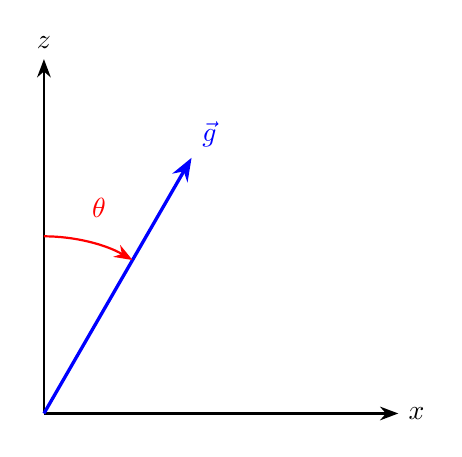
\begin{tikzpicture}[scale=1.5, >=Stealth]
	  			% Assi
	  			\draw[->, thick] (0,0) -- (3,0) node[right] {$x$};
	  			\draw[->, thick] (0,0) -- (0,3) node[above] {$z$};

	  			\draw[->, very thick, blue] (0,0) -- (60:2.5) node[above right] {$\vec{g}$};

	  			\draw[->, red, thick] (0,1.5) arc (90:60:1.5);

	  			\node[red] at (75:1.8) {$\theta$};
	  		\end{tikzpicture}
	  	\end{minipage}
	  	\hfill 
	  	\begin{minipage}{0.45\textwidth}
	  		\centering
	  		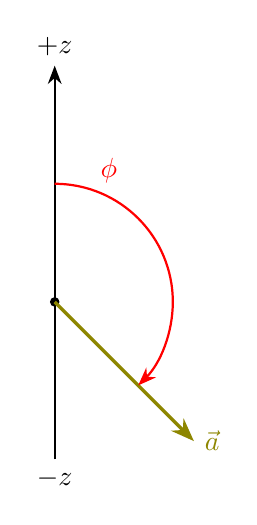
\begin{tikzpicture}[scale=1.0, >=Stealth]
	  			\draw[->, thick] (0,-2) -- (0,3) node[above] {$+z$};
	  			\node[below] at (0,-2) {$-z$};
	  			\filldraw (0,0) circle (1.5pt);
.
	  			\draw[->, very thick, olive] (0,0) -- (-45:2.5) node[right] {$\vec{a}$};

	  			\draw[->, red, thick] (0,1.5) arc (90:-45:1.5);

	  			\node[red] at (67.5:1.8) {$\phi$};
	  		\end{tikzpicture}
	  	\end{minipage}
	  \end{figure}
	  
	  \begin{gather}
	  	g_z = \cos{(\theta)} \quad ; \quad g_x = \sin{(\theta)} \label{eq:gz_gx_geom_def} \\
	  	g_0 = \cos{(\phi/2)} \quad ; \quad g_1 = \sin{(\phi/2)} \label{eq:g0_g1_geom_def} \\
	  	\text{so that} \quad g_0^2 - g_1^2 = \cos{(\phi)} \quad ; \quad 2g_0g_1 = \sin{(\phi)} \notag
	  \end{gather}
	  
	  In this way we can reformulate :
	  \begin{gather}
	  	g_{z}\left(g_{0}^{2} - g_{1}^{2} \right) + 2 g_{1} g_{0} g_{x} = 0 \notag \\
	  	\cos{(\theta)}\cos{(\phi)} + \sin{(\theta)}\sin{(\phi)} = 0 \notag \\
	  	\cos{(\theta - \phi)} = 0 \notag \\
	  	\theta - \phi = \frac{\pi}{2} \quad \rightarrow \quad \theta = \frac{\pi}{2} + \phi
	  	\label{eq:g_equivalnce_geom_sol}
	  \end{gather}
	  
	  Geometrically, this signifies that purely dissipative dynamics, in the Lindblad form, emerge only when the direction of the Collisional Interaction vector is perpendicular to the Ancilla's polarization vector on the Bloch sphere.

	  \newpage
	
	  To recover the two limits we have to set: 
	  
	  \begin{itemize}
	  	\item Quantum Jump limit : $ g_z = 0 , g_x = 1 \, ; \, g_0 = 1 , g_1 = 0 \, ; \, \theta = 90° , \phi = 0° $
	  	\item Diffusive limit : $ g_z = 1 , g_x = 0 \, ; \, g_0 = 1/\sqrt{2} , g_1 = 1/\sqrt{2} \, ; \, \theta = 0° , \phi = 90° $
	  \end{itemize}
	  
	  It is worth noting that the resulting Master Equation that lead to the Lindblad form with $ \mathcal{L}_k = \sigma_{z} $ describes a Pure Dephasing dynamic, where the Collisional environment destroys the quantum Coherence of the system, without inducing population transfer (energy relaxation).

	  \begin{equation}
	  	\dot{\rho_S} = \Gamma \left(\sigma_{z} \rho_S \sigma_{z} - \rho_S \right) \quad \text{Pure Dephasing}
	  	\label{eq:lindblad_pure_deph_recover}
	  \end{equation}
	  
	  It's possible to redefine the $ \mathcal{M} $ operators using the relations between the \textit{g} parameters :
	  \begin{align}
	  	\mathcal{M}_0 &= g_0 \cos(c_j \Delta t) \mathbb{I}^{j} + i g_1 \sin(c_j \Delta t) \sigma_{z}^{j} \label{eq:M0_simplified} \\
	  	\mathcal{M}_1 &= g_1 \cos(c_j \Delta t) \mathbb{I}^{j} - i g_0 \sin(c_j \Delta t) \sigma_{z}^{j} \label{eq:M1_simplified}
	  \end{align}
	  
	  and on the other way : 
	  \begin{align}
	  	\mathcal{M}_0 &= \sqrt{\frac{1+g_x}{2}} \cos(c_j \Delta t) \mathbb{I}^{j} + i \sqrt{\frac{1-g_x}{2}} \sin(c_j \Delta t) \sigma_{z}^{j} \\
	  	\mathcal{M}_1 &= \sqrt{\frac{1-g_x}{2}} \cos(c_j \Delta t) \mathbb{I}^{j} - i \sqrt{\frac{1+g_x}{2}} \sin(c_j \Delta t) \sigma_{z}^{j}
	  \end{align}	  
	  	  
	  \subsubsection{Focus on the $ 3^{rd} $ term}
	  Let's check what happens if we don't erase the last term in Eq.46 
	  
	  \begin{equation}
	  	i \Big( g_{z}\left(g_{0}^{2} - g_{1}^{2} \right) + 2 g_{1} g_{0} g_{x} \Big) \cos{\left(c_j \Delta t \right)} \sin{\left(c_j \Delta t \right)} \Big[\rho_S , \sigma_{z} \Big]
	  	\label{eq:3_term}
	  \end{equation}
	  \\
	  As seen so far in section 2.2.3 we can recover the complete form of  
	  \begin{equation}
		\rho_S' = \rho_S (t + \Delta t) = \mathcal{U}_{tot}(\Delta t) \rho_S (t) = \exp{\left[-i \, \left(\mathcal{H}_{Exc} + \mathcal{H}_{Coll} \right) \, \Delta t \right]} \rho_S (t)
		\label{eq:rho_S_LVN_comp_evo}
	  \end{equation}\\	  
	  by Trottarization of the $ \mathcal{U}_{tot} = e^{-i \, \mathcal{H}_{Exc} \, \Delta t } \, e^{-i \, \mathcal{H}_{Coll} \, \Delta t }  $ (with an error $ \mathcal{O}\left(\Delta t^2\right) $) .\\
	  So that we can sequently apply the two exponential operator, in particular we already know the result given by the Collsional term, i.e. Eq.46 at which we can apply the Exciton term; but first we need to explicit its $ \lim{\Delta t \rightarrow 0} $ : 
	  
	  \begin{equation}
	  	\lim\limits_{\Delta t \rightarrow 0} \, \rho_S' = \rho_S + c_{j}^{2} \Delta t ^{2} \left( \sigma_{z} \rho_S \sigma_{z} - \rho_S \right) + i \Big( g_{z}\left(g_{0}^{2} - g_{1}^{2} \right) + 2 g_{1} g_{0} g_{x} \Big) c_j \Delta t [\rho_S , \sigma_{z} \Big] 
	  	\label{eq:lim0_comp_rho_s}
	  \end{equation} 
	  
	   Since : \begin{itemize}
	   \item $ \cos{\left(c_j \Delta t \right)}^{2} \approx 1 - c_{j}^{2} \Delta t ^{2} $
	   \item $ \sin{\left(c_j \Delta t \right)}^{2} \approx c_{j}^{2} \Delta t ^{2} $
	   \item $ \cos{\left(c_j \Delta t \right)} \sin{\left(c_j \Delta t \right)} \approx 1 \cdot c_j \Delta t  $
	   \end{itemize}
	   Now defining $ \Gamma_{j} = c_{j}^{2} \Delta t $ and $ \mathcal{K} = \Big( g_{z}\left(g_{0}^{2} - g_{1}^{2} \right) + 2 g_{1} g_{0} g_{x} \Big) c_j $ , we can rewrite more comfortably : 
	   \begin{equation}
	   	\rho_S' = \rho_S + \Gamma_{j} \Delta t \left( \sigma_{z} \rho_S \sigma_{z} - \rho_S \right) + i \mathcal{K} \Delta t \Big[ \rho_S , \sigma_{z} \Big]
	   	\label{eq:compact_rho_S_evo}
	   \end{equation}
	   
	   We can now apply the evolution due to the $ \mathcal{H}_{Exc} $ which in the first order approximation reduces to the Liouville - von Neumann equation : 

	   \begin{gather}
	   	\rho_S (t + \Delta t) = e^{-i \, \mathcal{H}_{Exc} \Delta t} \rho_S' e^{\, i \, \mathcal{H}_{Exc} \Delta t} \approx \rho_S' - i \Big[\mathcal{H}_{Exc} , \rho_S' \Big] \Delta t \notag \\
	   	= \rho_S' - i \Big[ \mathcal{H}_{Exc} \, , \, \rho_S + \Gamma_{j} \Delta t \left( \sigma_{z} \rho_S \sigma_{z} - \rho_S \right) + i \mathcal{K} \Delta t \Big[ \rho_S , \sigma_{z} \Big] \Big] \Delta t
	   	\label{eq:compact_complete_rho_S_evo}
	   \end{gather} 
	   
	   Considering again $ \lim \Delta t \rightarrow 0 $ we can neglect the term quadratic in $ \Delta t $
	   
	   \begin{gather}
	   	\rho_S (t + \Delta t) \approx \rho_S + \Gamma_{j} \Delta t \left( \sigma_{z} \rho_S (t) \sigma_{z} - \rho_S (t) \right) - i \mathcal{K} \Delta t \Big[ \sigma_{z} , \rho_S (t) \Big] - i \Big[ \mathcal{H}_{Exc} \, , \, \rho_S (t) \Big] \notag \\
	   	\frac{\rho_S (t + \Delta t) - \rho_S (t)}{\Delta t} \approx \Gamma_{j} \left( \sigma_{z} \rho_S \sigma_{z} - \rho_S \right) - i \Big[ \left( \mathcal{H}_{Exc} + \mathcal{K} \sigma_z \right), \rho_S \Big] \notag \\
	   	\dot{\rho_S} = \Gamma_{j} \left( \sigma_{z} \rho_S \sigma_{z} - \rho_S \right) - i \Big[ \left( \mathcal{H}_{Exc} + \mathcal{K} \sigma_z \right), \rho_S \Big]
	   	\label{eq:final_complete_form_rho_S_evo}
	   \end{gather}
	   
	   Remembering that $ \mathcal{K} = \Big( g_{z}\left(g_{0}^{2} - g_{1}^{2} \right) + 2 g_{1} g_{0} g_{x} \Big) c_j $ derives from the $ 3^{rd} $ term in Eq.46 it's clear that this term act as a shift in the Energy of the system's site \{ Lamb Shift ?\}. \\
	   But we need to be careful since we have a $ c_j = \sqrt{\Gamma_j / \Delta t} $ in the $ \mathcal{K} $ definition and applying the $ \lim \Delta t \rightarrow 0 $ it would diverge. \\
	   To get around this problem we can redefine the components of the direction of $ \mathcal{H}_{Coll} $ as function of $ \Delta t $ :
	   
	   \begin{equation}
	   	g_z = \Gamma_{z} \sqrt{\Delta t} \quad ; \quad g_x = \Gamma_{x} \sqrt{\Delta t}
	   	\label{eq:gz_gx_reformulation}
	   \end{equation}
	   
	   so that Eq.40 becomes
	   \begin{align}
	   	\sqrt{g_{z}^{2} + g_{x}^{2}} = \sqrt{\Gamma_{z}^{2} + \Gamma_{x}^{2} } \sqrt{\Delta t} = 1
	   	\label{eq:geom_constrain}
	   \end{align}
	   
	   and $ \mathcal{K} $ becomes independent from $ \Delta t $
	   
	   \begin{align}
		\mathcal{K} &= \frac{\sqrt{\Gamma_{j}}}{\cancel{\sqrt{\Delta t}}} \cdot \cancel{\sqrt{\Delta t}} \left( \Gamma_{z}\left(g_{0}^{2} - g_{1}^{2} \right) + 2 g_{1} g_{0} \Gamma_{x}\right) \notag \\
		&= \sqrt{\Gamma_{j}} \left( \Gamma_{z}\left(g_{0}^{2} - g_{1}^{2} \right) + 2 g_{1} g_{0} \Gamma_{x}\right)
		\label{eq:K_term_refomrulation}
	   \end{align}
	   
	   This solution is coherent with the definition used for $ c_j = \sqrt{\Gamma_j / \Delta t} $ and the Collisional Hamiltonian becomes :
	    
	   \begin{equation}
	   	\mathcal{H}_{Coll} = \sqrt{\Gamma_{j}} \, \sigma_{z}^{j} \otimes \left( \Gamma_{z} \sigma_{z}^{a_j} + \Gamma_{x} \sigma_{x}^{a_j} \right)
	   	\label{eq:H_coll_refomrulation}
	   \end{equation}
	   	   
	   \subsubsection{Probability of measuring the Ancilla's states}
	   
	   After the collision the Ancilla could be either in state $ \ket{0_a} $ or $ \ket{1_a} $ with a finite probability which is generally given by:
	   
	   \begin{align}
	   	P_{0_{a}} = Tr_{S} \left[\braket{0_a|\Psi'}\braket{\Psi'|0_a} \right] \\
	   	P_{1_{a}} = Tr_{S} \left[\braket{1_a|\Psi'}\braket{\Psi'|1_a} \right]
	   \end{align}
	   
	   To evaluate this values we first redefine the operators $ \mathcal{M}_{0} $ and $ \mathcal{M}_{1} $ using the value :
	   \begin{align}
	   	a_{0} = g_{0} \cos{\left(c_{j}\Delta t\right)} \quad ; \quad b_{0} = \left(g_{0} g_{z} + g_{1}g_{x} \right) \sin{\left(c_{j}\Delta t\right)} \label{eq_a0_b0_def} \\
	   	a_{1} = g_{1} \cos{\left(c_{j}\Delta t\right)} \quad ; \quad b_{1} = \left(g_{0} g_{x} - g_{1}g_{z} \right) \sin{\left(c_{j}\Delta t\right)} \label{eq_a01b1_def}
	   \end{align}
	   so that : 
	   \begin{align}
	   	\mathcal{M}_{0} = a_{0} \mathbb{I}^{j} -i b_{0} \sigma_{z}^{j} \quad ; \quad \mathcal{M}_{0}^{\dagger} = a_{0} \mathbb{I}^{j} + i b_{0} \sigma_{z}^{j} \label{eq_M0_def} \\
	   	\mathcal{M}_{1} = a_{1} \mathbb{I}^{j} -i b_{1} \sigma_{z}^{j} \quad ; \quad \mathcal{M}_{1}^{\dagger} = a_{1} \mathbb{I}^{j} + i b_{1} \sigma_{z}^{j}
	   	\label{eq_M1_def}
	   \end{align}
	   
	   If we expand Eq.\ref{eq:MO_M1_rho_int} using this definition :
	   \begin{align}
	   	\rho' &= \ket{\Psi'}\bra{\Psi'} = \mathcal{M}_{0} \rho_S \mathcal{M}_{0}^{\dagger} \otimes \ket{0_a}\bra{0_a} + \mathcal{M}_{1} \rho_S \mathcal{M}_{1}^{\dagger} \otimes \ket{1_a} \bra{1_a} \notag \\
	   	& \quad + \mathcal{M}_{0} \rho_S \mathcal{M}_{1}^{\dagger} \otimes \ket{0_a} \bra{1_a} + \mathcal{M}_{1} \rho_S \mathcal{M}_{0}^{\dagger} \otimes \ket{1_a} \bra{0_a} \notag \\
	   	& = \left(a_{0} \mathbb{I}^{j} - i b_{0} \sigma_{z}^{j}\right) \ket{\Psi_{S}}\bra{\Psi_{S}} \left(a_{0} \mathbb{I}^{j} + i b_{0} \sigma_{z}^{j}\right) \otimes \ket{0_{a}} \bra{0_{a}} \notag \\
	   	& + \left(a_{1} \mathbb{I}^{j} - i b_{1} \sigma_{z}^{j}\right) \ket{\Psi_{S}}\bra{\Psi_{S}} \left(a_{1} \mathbb{I}^{j} + i b_{1} \sigma_{z}^{j}\right) \otimes \ket{1_{a}} \bra{1_{a}} \notag \\
	   	& + \left(a_{0} \mathbb{I}^{j} - i b_{0} \sigma_{z}^{j}\right) \ket{\Psi_{S}}\bra{\Psi_{S}} \left(a_{1} \mathbb{I}^{j} + i b_{1} \sigma_{z}^{j}\right) \otimes \ket{0_{a}} \bra{1_{a}} \notag \\
	   	& + \left(a_{1} \mathbb{I}^{j} - i b_{1} \sigma_{z}^{j}\right) \ket{\Psi_{S}}\bra{\Psi_{S}} \left(a_{0} \mathbb{I}^{j} + i b_{0} \sigma_{z}^{j}\right) \otimes \ket{1_{a}} \bra{0_{a}} \notag \\
	   	& = \Big[ \left|a_{0}\right|^{2} \ket{\Psi_{S}}\bra{\Psi_{S}} + \left|b_{0}\right|^{2} \sigma_{z}^{j}\ket{\Psi_{S}}\bra{\Psi_{S}}\sigma_{z}^{j} + i a_{0}b_{0}\ket{\Psi_{S}}\bra{\Psi_{S}}\sigma_{z}^{j} -  i a_{0}b_{0} \sigma_{z}^{j} \ket{\Psi_{S}}\bra{\Psi_{S}} \Big] \otimes \ket{0_{a}} \bra{0_{a}} \notag \\
	   	& + \Big[ \left|a_{1}\right|^{2} \ket{\Psi_{S}}\bra{\Psi_{S}} + \left|b_{1}\right|^{2} \sigma_{z}^{j}\ket{\Psi_{S}}\bra{\Psi_{S}}\sigma_{z}^{j} + i a_{1}b_{1}\ket{\Psi_{S}}\bra{\Psi_{S}}\sigma_{z}^{j} -  i a_{1}b_{1} \sigma_{z}^{j} \ket{\Psi_{S}}\bra{\Psi_{S}} \Big] \otimes \ket{1_{a}} \bra{1_{a}} \notag \\
	   	& + \Big[ a_{0} a_{1} \ket{\Psi_{S}}\bra{\Psi_{S}} + b_{0} b_{1}  \sigma_{z}^{j}\ket{\Psi_{S}}\bra{\Psi_{S}}\sigma_{z}^{j} + i a_{0}b_{1}\ket{\Psi_{S}}\bra{\Psi_{S}}\sigma_{z}^{j} -  i a_{1}b_{0} \sigma_{z}^{j} \ket{\Psi_{S}}\bra{\Psi_{S}} \Big] \otimes \ket{0_{a}} \bra{1_{a}} \notag \\
	   	& + \Big[ a_{1} a_{0} \ket{\Psi_{S}}\bra{\Psi_{S}} + b_{1} b_{0}  \sigma_{z}^{j}\ket{\Psi_{S}}\bra{\Psi_{S}}\sigma_{z}^{j} + i a_{1}b_{0}\ket{\Psi_{S}}\bra{\Psi_{S}}\sigma_{z}^{j} -  i a_{0}b_{1} \sigma_{z}^{j} \ket{\Psi_{S}}\bra{\Psi_{S}} \Big] \otimes \ket{1_{a}} \bra{0_{a}} \notag
	   \end{align}
	   Now we can calculate :
	   \begin{align}
		P_{0_{a}} & = Tr_{S} \left[\braket{0_a|\Psi'}\braket{\Psi'|0_a} 	\right] \notag \\
		& = Tr_{S} \Big[ \left|a_{0}\right|^{2} 	\ket{\Psi_{S}}\bra{\Psi_{S}} + \left|b_{0}\right|^{2} \sigma_{z}^{j} \ket{\Psi_{S}}\bra{\Psi_{S}} \sigma_{z}^{j} + i a_{0}b_{0}\ket{\Psi_{S}}\bra{\Psi_{S}} \sigma_{z}^{j} -  i a_{0}b_{0} \sigma_{z}^{j} \ket{\Psi_{S}}\bra{\Psi_{S}} \Big] \notag \\
		& = \left|a_{0}\right|^{2} Tr_{S} \Big[ 	\ket{\Psi_{S}}\bra{\Psi_{S}} \Big] + \left|b_{0}\right|^{2} Tr_{S} \Big[ \sigma_{z}^{j} \ket{\Psi_{S}}\bra{\Psi_{S}} \sigma_{z}^{j} \Big] \notag \\
		& \quad + i \,a_{0} b_{0} \, Tr_{S} \Big[ 	\ket{\Psi_{S}}\bra{\Psi_{S}} \sigma_{z}^{j} \Big] - i \, a_{0} b_{0} \, Tr_{S} \Big[ \sigma_{z}^{j} \ket{\Psi_{S}}\bra{\Psi_{S}} \Big] \notag \\
		& \big(\text{remembering that} \quad Tr \left[ABC\right] = Tr 	\left[CAB\right] \quad \text{and} \quad \sigma_{z} \sigma_{z} = \mathbb{I} \big) \notag \\
		& = \left|a_{0}\right|^{2} Tr_{S} \Big[ 	\ket{\Psi_{S}}\bra{\Psi_{S}} \Big] + \left|b_{0}\right|^{2} Tr_{S} \Big[  \ket{\Psi_{S}}\bra{\Psi_{S}} \Big] \notag \\
		& \quad + \cancel{i \,a_{0} b_{0} \, Tr_{S} \Big[ \sigma_{z}^{j} 	\ket{\Psi_{S}}\bra{\Psi_{S}} \Big]} \cancel{- i \, a_{0} b_{0} \, Tr_{S} \Big[ \sigma_{z}^{j} \ket{\Psi_{S}}\bra{\Psi_{S}} \Big]} \notag \\
		P_{0_{a}} & = \left|a_{0}\right|^{2} + \left|b_{0}\right|^{2} = 	g_{0}^{2} \cos^{2}{\left(c_{j}\Delta t\right)} + \left(g_{0} g_{z} + g_{1}g_{x} \right)^{2} \sin^{2}{\left(c_{j}\Delta t\right)} \label{eq_P0_value} \\
		\notag \\
	    & \text{and the same for :} \notag \\
	    \notag \\
	  	P_{1_{a}} &= \left|a_{1}\right|^{2} + \left|b_{1}\right|^{2} = 	g_{1}^{2} \cos^{2}{\left(c_{j}\Delta t\right)} + \left(g_{0} g_{x} - g_{1}g_{z} \right)^{2} \sin^{2}{\left(c_{j}\Delta t\right)} \label{eq_P1_value}
	   \end{align}
	   
	   Or in another formulation : 
	   \begin{align}
	   	P_{0_a} & = g_0^2 \cos^2(c_j \Delta t) + g_1^2 \sin^2(c_j \Delta t) \\
	   	P_{1_a} & = g_1^2 \cos^2(c_j \Delta t) + g_0^2 \sin^2(c_j \Delta t)
	   \end{align}
	   
	   So setting the \textit{g} parameter directly defines the probability of measuring a different Ancilla's state; we could check if this definition lead back to the probability obtained in the Quantum Jump and Coherent limit:
	  
	   \begin{itemize}
	  		\item QJ : $ g_z = 0 , g_x = 1 \, ; \, g_0 = 1 , g_1 = 0 \, ; \, \theta = 90° , \phi = 0° \rightarrow P_{0_{a}} = \cos^{2}{\left(c_{j}\Delta t\right)} \, ; \, P_{1_{a}} = \sin^{2}{\left(c_{j}\Delta t\right)} $
	  		\item Diff : $ g_z = 1 , g_x = 0 \, ; \, g_0 = 1/\sqrt{2} , g_1 = 1/\sqrt{2} \, ; \, \theta = 0° , \phi = 90° \rightarrow P_{0_{a}} = \frac{1}{2} \, ; \, P_{1_{a}} = \frac{1}{2} $
	   \end{itemize} 
		   
	   Now we could try to see how the probability of measuring the two different Ancilla's states changes varying the \textit{g} values, for example as function of the angle $ \theta $ (with $ \theta = \frac{\pi}{2} + \phi $) : 
	
	   \graphicspath{ {/home/francesco/Collisional_Methods/Results/Plot/Probability} }
	   \begin{figure}[H]
	   	\centering
	   	\includegraphics[width=0.7\textwidth]{{Prob(theta)}.png}
	   	\caption{Probability of measuring the two different Ancilla's states $\ket{0_{a}}$ and $\ket{1_{a}}$, as function of the $\theta$ angle, which defines the direction of the $\mathcal{H}_{\text{Coll}}$ respect to z axis}
	   	\label{fig:prob_theta}
	   \end{figure}
	
	   As observed, for $\theta = 90^\circ$ (Quantum Jump limit), the probability of measuring $\ket{0_{a}}$ is $P_{0_{a}}\approx 1$. This corresponds to the application of the identity operator $\mathbb{I}^{j}$ on the system's wf; conversely, the probability of measuring $\ket{1_{a}}$ is $P_{1_{a}}\approx 0$, which corresponds to the application of $\sigma_{z}^{j}$. 
	   
	   On the other hand, for $\theta = 0^\circ$ (Diffusional limit), both probabilities are approximately $1/2$. In this regime, the system's wf undergoes a continuous modification regardless of the outcome ($\ket{0_{a}}$ or $\ket{1_{a}}$), with the modification weighted by a small factor and differing by a sign.\\
	   
	   \newpage
	   
	   Now the question that arises is, if both the two unraveling has to give back the same average dynamic, but 
	   
	   \begin{itemize}
	   	\item in the QJ limit we have a small probability to apply a big change in the System's wf ;
	   	\item in the Diff. limit we always apply a variation to the System's wf but this produces a small change.
	   \end{itemize}
	   
	   Is it possible to quantify a quantity that defines the intensity of the variation applied to the System's wf after the collision? Is it possible to define it as a function of the \textit{g} parameters? And therefore, what would its behavior be with respect to the angle theta?
	  
	  \subsection{Focus on $\mathcal{M}_0$ and $\mathcal{M}_1$ operator}
	  \label{sub:focus_on_M0_M1}
	  Remember that:
	  \begin{align*}
	  	\mathcal{M}_0 &= g_0 \cos(c_j \Delta t) \mathbb{I}^{j} + i g_1 \sin(c_j \Delta t) \sigma_{z}^{j} \\
	  	\mathcal{M}_0^{\dagger} &= g_0 \cos(c_j \Delta t) \mathbb{I}^{j} - i g_1 \sin(c_j \Delta t) \sigma_{z}^{j} \\
	  	\mathcal{M}_1 &= g_1 \cos(c_j \Delta t) \mathbb{I}^{j} - i g_0 \sin(c_j \Delta t) \sigma_{z}^{j} \\
	  	\mathcal{M}_1^{\dagger} &= g_1 \cos(c_j \Delta t) \mathbb{I}^{j} + i g_0 \sin(c_j \Delta t) \sigma_{z}^{j} 
	  \end{align*}
	  Are this operators \textit{Unitary} ?
	  \begin{align}
	  	\mathcal{M}_0^{\dagger}\mathcal{M}_0 = [g_0^2 \cos^2(c_j \Delta t) + g_1^2 \sin^2(c_j \Delta t)] \mathbb{I} \\
	  	\mathcal{M}_1^{\dagger}\mathcal{M}_1 = [g_1^2 \cos^2(c_j \Delta t) + g_0^2 \sin^2(c_j \Delta t)] \mathbb{I}
	  \end{align}
	  
	  Calculation of those quantities that defines how much the \textit{wf} is similar to itself after the evolution via $ \mathcal{M}_0 $ and $ \mathcal{M}_1 $ (related to the \textit{wf} Modification Intensity), defined by the overlap of the two \textit{wf}:
	  \begin{align}
	  	\left| \braket{\Psi_{S}^{PRE} | \Psi_{S}^{POST}}_{\mathcal{M}_{0}} \right|^2 = \left| \bra{\Psi_{S}^{PRE}}\mathcal{M}_0 \ket{\Psi_{S}^{PRE}} \right|^2 &= g_0^2 \cos^2{\left(c_j \Delta t \right)} + g_1^2 \sin^2{\left(c_j \Delta t \right)} \left| \braket{\sigma_{z}} \right|^2 \label{eq:fidelity_M0} \\
	  	\left| \braket{\Psi_{S}^{PRE} | \Psi_{S}^{POST}}_{\mathcal{M}_{1}} \right|^2 = \left| \bra{\Psi_{S}^{PRE}}\mathcal{M}_1 \ket{\Psi_{S}^{PRE}} \right|^2 &= g_1^2 \cos^2{\left(c_j \Delta t \right)} + g_0^2 \sin^2{\left(c_j \Delta t \right)} \left| \braket{\sigma_{z}} \right|^2 \label{eq:fidelity_M1}
	  \end{align}
	  where 
	  \begin{equation*}
		\left| \braket{\sigma_{z}} \right|^2 = \left| \bra{\Psi_{S}^{PRE}} \sigma_{z} \ket{\Psi_{S}^{PRE}} \right|^2
	  \end{equation*}
	  Those quantity corresponds exactly to the definition of \textit{Fidelity} in the case of Pure States : 
	  \begin{gather}
	  	\mathcal{F}_{\mathcal{M}_{0}} = \left| \braket{\Psi_{S}^{PRE} | \Psi_{S}^{POST}}_{\mathcal{M}_{0}} \right|^2 \\
	  	\mathcal{F}_{\mathcal{M}_{1}} = \left| \braket{\Psi_{S}^{PRE} | \Psi_{S}^{POST}}_{\mathcal{M}_{1}} \right|^2 
	  \end{gather}
	  So that the quantity related to the difference between the two \textit{wf} before and after the collision is :
	  \begin{align}
	  	nome da inventare = 1 - \left| \braket{\Psi_{S}^{PRE} | \Psi_{S}^{POST}}_{\mathcal{M}_{0}} \right|^2 \\
	  	nome da inventare = 1 - \left| \braket{\Psi_{S}^{PRE} | \Psi_{S}^{POST}}_{\mathcal{M}_{1}} \right|^2
	  \end{align}
	  As we could see this quantities depends on the form of the \textit{wf}, for different time steps and different trajectories.
	  So we need to evaluate this for different values of $ \left| \braket{\sigma_{z}^{j}} \right|^2 $ in different unraveling schemes. For this purpose it might be useful to rephrase Eq.\eqref{eq:fidelity_M0} and Eq.\eqref{eq:fidelity_M0} as follows:
	  
	  \begin{equation}
		  	c = \cos^{2} \left( c_{j} \Delta t \right) \quad ; \quad s_{z} = \left| \braket{\sigma_{z}} \right|^2 = \left| \bra{\Psi_{S}} \sigma_{z} \ket{\Psi_{S}} \right|^2
	  \end{equation}
	  \begin{align}
	  	\left| \braket{\Psi_{S}^{PRE} | \Psi_{S}^{POST}}_{\mathcal{M}_{0}} \right|^2 = g_{0}^{2} \left[ c - s_{z} \left(1 - c \right) \right] + s_{z} \left(1 - c \right) \label{eq:fidelity_M0_ref} \\ 
	  	\left| \braket{\Psi_{S}^{PRE} | \Psi_{S}^{POST}}_{\mathcal{M}_{1}} \right|^2 = g_{0}^{2} \left[ s_{z} \left(1 - c \right) - c \right] + c \label{eq:fidelity_M1_ref}
	  \end{align}
	  It's important to point out that the value of $ c = \cos^{2} \left( c_{j} \Delta t \right) \approx 1 $ due to the chosen parameters $ c_j $ and $ dt $. This gives consequentially $ 1 - c = \sin^{2} \left( c_{j} \Delta t \right) \approx 3.046 \times 10^{-10} \approx 0 $, which is the coefficient that weights $ \left| \braket{\sigma_{z}} \right|^2 $, that could essentially be considered irrelevant.
	  Moreover it's important to specify what effectively we are calculating with $ \left| \braket{\sigma_{z}} \right|^2 = \left| \bra{\Psi_{S}} \sigma_{z} \ket{\Psi_{S}} \right|^2 $, where:
	  \begin{gather}
	  	\sigma_{z} = \sigma_{z}^{1} \otimes \mathbb{I} + \mathbb{I} \otimes \sigma_{z}^{2}
	  \end{gather}
	  so that
	  \begin{align}
		\left| \braket{\sigma_{z}} \right| = P_{01} - P_{10} - \left( P_{01} - P_{10} \right) = 0
	  \end{align}
	  so the second term of Eq.\ref{eq:fidelity_M0} and Eq.\ref{eq:fidelity_M1} vanishes definitely.
	  
	  Anyway it could be interesting to evaluate the values of $ \left| \braket{\sigma_{z}}^{j} \right|^2 = \left| \bra{\Psi_{S}} \sigma_{z}^{j} \ket{\Psi_{S}} \right|^2 $ for the single site, comparing it for different unraveling scheme, in order to see if this could give different frequency of "\textit{site visiting}", i.e. if for different unraveling one of the two site is more populated during the dynamic.
	  
	  First, since $ \left| \braket{\sigma_{z}} \right| \in [-1,1] $ and $ g_{0} \in [0,1] $, it's possible to plot the value of Eq.\ref{eq:fidelity_M0} and Eq.\ref{eq:fidelity_M1} as a function of $ g_{0} $ and $ \left| \braket{\sigma_{z}}^{j} \right| $ : 
	   \graphicspath{ {/home/francesco/Collisional_Methods/Results/Plot/Probability/Fidelity} }
	  \begin{figure}[H]
	  	\centering
	  	
\includegraphics[width=0.9\textwidth]{Fidelity_g0_Sz.png}
	  	\caption{Fidelity as a function of $ \left| \braket{\sigma_{z}^{j}} \right| $ and $ g_0 $}
	  	\label{fig:Fidelity_g0_Sz}
	  \end{figure}
	  Taking some slices of the 3D plot we see that : 
	  \graphicspath{ {/home/francesco/Collisional_Methods/Results/Plot/Probability/Fidelity} }
	  \begin{figure}[H]
	  	\centering
	  	\includegraphics[width=0.6\textwidth]{Fidelity_g0.png}
	  	\caption{Fidelity as a function of only $ g_0 $. This result is approximately the same for every different value of $ \left| \braket{\sigma_{z}^{j}} \right| $ }
	  	\label{fig:Fidelity_g0}
	  \end{figure}
	  \graphicspath{ {/home/francesco/Collisional_Methods/Results/Plot/Probability/Fidelity/} }
	  \begin{figure}[H]
	  	\centering
	  	% First Pannel(a)
	  	\begin{subfigure}[b]{0.48\textwidth}
	  		\centering
	  		
\includegraphics[width=\textwidth]{Fidelity_Sz_1.png}
	  		\caption{}
	  		\label{fig:Fidelity_Sz_1}
	  	\end{subfigure}
	  	\hfill
	  	% Second Pannel (b)
	  	\begin{subfigure}[b]{0.48\textwidth}
	  		\centering
	  		
\includegraphics[width=\textwidth]{Fidelity_Sz_2.png}
	  		\caption{}
	  		\label{fig:Fidelity_Sz_2}
	  	\end{subfigure}
	  	
	  	\caption{Fidelity as a function of only $\left| \braket{\sigma_{z}^{j}} \right|$ for different values of $g_0$. Panel (a) shows the results for $ g_{0} = 0.82 $, while panel (b) displays the outcome for $ g_{0} = 0.60 $.}
	  	\label{fig:Fidelity_Sz}
	  \end{figure}
	  
	  This plots gives confirmation of the fact that the second term proportional to $\left| \braket{\sigma_{z}^{j}} \right|$ it's negligible, in fact we have the same results for different value of $\left| \braket{\sigma_{z}^{j}} \right|$ in Fig.\ref{fig:Fidelity_g0} and there's no quadratic dependence on $\left| \braket{\sigma_{z}^{j}} \right|$ in Fig.\ref{fig:Fidelity_Sz}, where the Fidelity essentially are constants equal to :
	  \begin{gather}
	  	\mathcal{F}_{\mathcal{M}_{0}} \approx g_{0}^{2} \cos^{2}\left(c_{j} \Delta t \right) \\
	  	\mathcal{F}_{\mathcal{M}_{1}} \approx \left(1 - g_{0}^{2}\right) \cos^{2}\left(c_{j} \Delta t \right)
	  \end{gather}
	  
	  Another important thing to check is the distribution of $\left| \braket{\sigma_{z}^{j}} \right|$ and $\left| \braket{\sigma_{z}^{j}} \right|^2$ recorded during the dynamics for different \textit{Unraveling Scheme}. With this results we should see if different unraveling gives different values of the quantities described above, i.e. some states are more visited or one site is more populated during the trajectories. This could directly affect the fidelity, which also depends, and in a practically irrelevant way, on $\left| \braket{\sigma_{z}^{j}} \right|$ which in turn depends on the sampled state at each time step (for example, eigenstates of $ \sigma_{z} $ would have $ \mathcal{F} = 1 $, i.e. rotation around the z-axis is irrelevant).
	  
	  At this purpose for every Trajectory and at every time step th values of $\left| \braket{\sigma_{z}^{1}} \right|$ and $\left| \braket{\sigma_{z}^{2}} \right|$ were calculated and stored in two matrices \texttt{Sz\_matrix\_1(n\_times, N\_traj)} and \texttt{Sz\_matrix\_2(n\_times, N\_traj)}; notice that :
	  \begin{gather}
			\left| \braket{\sigma_{z}^{1}} \right| = \left| \bra{\Psi_{S}} \sigma_{z}^{1} \ket{\Psi_{S}} \right| \quad \text{where} \quad \sigma_{z}^{1} = \sigma_{z} \otimes \mathbb{I} \\
			\left| \braket{\sigma_{z}^{2}} \right| = \left| \bra{\Psi_{S}} \sigma_{z}^{2} \ket{\Psi_{S}} \right| \quad \text{where} \quad \sigma_{z}^{2} = \mathbb{I} \otimes \sigma_{z}
	  \end{gather}
	  Once we've obtained \texttt{Sz\_matrix\_1(n\_times, N\_traj)} and \texttt{Sz\_matrix\_2(n\_times, N\_traj)}, it's possible to calculate the average value over the trajectories and then the square values, that enter in Eq.\ref{eq:fidelity_M0} and Eq.\ref{eq:fidelity_M1}. Finally, the temporal distribution of these results was visualized using histograms : 
	  
	  \graphicspath{ {/home/francesco/Collisional_Methods/Results/Plot/Probability/Sx_Sy_Sz/} }
	  
	  \begin{figure}[H]
	  	\centering
	  	% First Panel(a)
	  	\begin{subfigure}[b]{0.48\textwidth}
	  		\centering
	  		
\includegraphics[width=\textwidth]{Sz_distribution_intermediate.png}
	  		\caption{}
	  		\label{fig:Sz_avg}
	  	\end{subfigure}
	  	\hfill
	  	% Second Panel(b)
	  	\begin{subfigure}[b]{0.48\textwidth}
	  		\centering
	  		
\includegraphics[width=\textwidth]{Sz_square_distribution_intermediate.png}
	  		\caption{}
	  		\label{fig:Sz_square_avg}
	  	\end{subfigure}
	  	\caption{Distribution of $\left| \braket{\sigma_{z}^{1}} \right|$ in panel (a), and $\left| \braket{\sigma_{z}^{1}} \right|^2$ in panel (b), recorded during the dynamics and averaged over 10,000 trajectories.}
	  	\label{fig:Sz_distributions}
	  \end{figure}
	  
	  \begin{figure}[H]
	  	\centering
	  	% First Panel(a)
	  	\begin{subfigure}[b]{0.48\textwidth}
	  		\centering
	  		
\includegraphics[width=\textwidth]{Sz_distribution_close_to_90_deg.png}
	  		\caption{}
	  		\label{fig:Sz_avg_close_to_90}
	  	\end{subfigure}
	  	\hfill
	  	% Second Panel(b)
	  	\begin{subfigure}[b]{0.48\textwidth}
	  		\centering
	  		
\includegraphics[width=\textwidth]{Sz_square_distribution_close_to_90_deg.png}
	  		\caption{}
	  		\label{fig:Sz_square_avg_close_to_90}
	  	\end{subfigure}
	  	\caption{Distribution of $\left| \braket{\sigma_{z}^{1}} \right|$ in panel (a), and $\left| \braket{\sigma_{z}^{1}} \right|^2$ in panel (b), recorded during the dynamics and averaged over 10,000 trajectories, for angles close to 90°.}
	  	\label{fig:Sz_distributions_close_to_90_deg}
	  \end{figure}
	  
	  As expected the histograms give the same distribution for different unraveling scheme, which is centered in 0.0, since the \textit{Ensamble Average}, over the trajectories, reproduces the Lindblad distribution of $ \braket{\sigma_{z}^{j}} $, so since the dynamics of the site populatin is a dumped oscillation towards the value 0.5 and $ \braket{\sigma_{z}^{j}} \propto P_{10} - P_{01} $, values close to 0.0 should be sampled more often. Consequentially the squared values are just the squared positive part of the $ \braket{\sigma_{z}^{j}} $ distribution. 
	  
	  Notice that only $ \braket{\sigma_{z}^{j}} $ is calculated since this value i related to the single site, where in the \textit{Dephasing Dynamics} where only the excited states are populated, $ \braket{\sigma_{x}^{j}} = \braket{\sigma_{y}^{j}} = 0 $.
	  
	  plot istogrammi non mediati per singola traiettoria e calcolo varianza
	  
	  
\end{document}	